\documentclass{article}

\usepackage[utf8]{inputenc}

\usepackage{graphicx}
\usepackage{subcaption}
\usepackage{mathtools}
\usepackage{wrapfig}
\usepackage{graphicx}
\usepackage{subcaption}
\usepackage{mathtools}
\usepackage{wrapfig}
\usepackage{float}
\usepackage{gensymb}
\usepackage{caption}
\usepackage{geometry}
\usepackage{cite}

\DeclareMathOperator{\sech}{sech}
\DeclareMathOperator{\Tr}{Tr}

\usepackage{listings}
\usepackage{color}

\definecolor{codegreen}{rgb}{0,0.6,0}
\definecolor{codegray}{rgb}{0.5,0.5,0.5}
\definecolor{codepurple}{rgb}{0.58,0,0.82}
\definecolor{backcolour}{rgb}{0.95,0.95,0.92}
 
\lstdefinestyle{mystyle}{
    backgroundcolor=\color{backcolour},   
    %commentstyle=\color{codegreen},
    %keywordstyle=\color{magenta},
    numberstyle=\tiny\color{codegray},
    %stringstyle=\color{codepurple},
    basicstyle=\footnotesize,
    breakatwhitespace=false,         
    breaklines=true,                 
    captionpos=b,                    
    keepspaces=true,                 
    numbers=left,                    
    numbersep=5pt,                  
    showspaces=false,                
    showstringspaces=false,
    showtabs=false,                  
    tabsize=2
}


\lstset{style=mystyle}





\makeatletter
\renewcommand\paragraph{\@startsection{paragraph}{4}{\z@}%
	{-2.5ex\@plus -1ex \@minus -.25ex}%
	{1.25ex \@plus .25ex}%
	{\normalfont\normalsize\bfseries}}
\makeatother
\setcounter{secnumdepth}{4} % how many sectioning levels to assign numbers to
\setcounter{tocdepth}{4}    % how many sectioning levels to show in ToC in preamble





\geometry
{
  %body={6.5in, 8.5in},
  left=1.3in,%1.0in,
  right =1.3in,
  top=1.25in
}

\setlength{\parindent}{10ex}









%\begin{figure}[H]
%	\centering
%	\includegraphics[scale=0.2]{rhul_logo}
%\end{figure}








%chris help


%some questions in paper under help 



%folyers english 






%%%%%%%%%%%%%%%%to do%%%%%%%%%%%%%%%%%%%%%%%%%%%

%2make sure appendixes match the paper 



%%%%%%%%%%rewrite%%%%%%%%%%%%

%%%%%%%%%%finish%%%%%%%%%%%%%

%3create transformation program 

%4write conversion code.  parser, first step


%%%%%%%%%%%add%%%%%%%%%%%%%%%%%


%%%%%%%%%%%%side things%%%%%%%%%%%%%%
%5replace $'$ with \textsc{\char13}



%%%%%%%%%%%%%proof%%%%%%%%%%%%%%%%%% 

%sec 3
%sec 4
%sec 5
%sec 6
%sec 7
%sec 8


 
\begin{document} 
\title{Translating from Recurrence Relations to an Agent-Based Representation} 
\author{
\\
\\
Leo Carlos-Sandberg\\
Supervisor: Dr Christopher D. Clack\\
\\
\\
\\
\\
\\
\\
\\
\\
\\
\\
\\
\\
A dissertation submitted in partial fulfilment\\
 of the requirements for the degree of\\
 \textbf{MRes in Financial Computing}\\
 of the \\
 \textbf{University College London}.
 \\
 \\
 \\
 \\
 \\
 Department of Computer Science\\
 University College London
 \\
 \\} 
\maketitle 

\newpage
I, Leo Carlos-Sandberg, confirm that the work presented in this dissertation is my own. Where information has been derived from other sources, I confirm that this has been indicated in the dissertation. The report may be freely copied and distributed provided the source is explicitly acknowledged.

\newpage
\begin{abstract}
\noindent {\it 
This dissertation investigates a process to increase the acceptance of agent-based models by translation from recurrence relation models. The work presented in this dissertation is designed to combat two main aspects that hinder the up take in agent-based models: a lack of a model-wide formalism, and a lack of familiarity to those unaccustomed to the technique. 

The importance of this work relates in particular to the field of economics, where agent-based models are yet to become widely accepted. This lack of acceptance leads to an absence of work based on agent-based models in top economics journals. This creates a problem for modelling complex systems and emergent behaviour, as agent-based models are in many cases a natural modelling technique for these systems, due in part to their message passing behaviour.  

The process presented in this dissertation is to create an agent-based model equivalent to a recurrence relation model. Recurrence relation models are both widely accepted and have a model-wide formalisation. Creating an equivalence between these two models allows for the recurrence relation model to give the agent-based model both a formalisation and a familiar representation, for economists.       

This work comprises the creation of a bespoke recurrence relation language, the design of step-by-step translation between the models, and a numeric testing of the equivalence of these models. 

The bespoke recurrence relation language presented in this work allows for an experiment involving complex and interacting systems to be laid out in a clear manner, using recurrence relations. 

A design for an eight-step translation that turns an experiment written in the bespoke recurrence relation language into an agent-based model is given. 

The agent-based model created in this translation is shown to be numerically equivalent to the initial recurrence relation model, for a number of starting values. Each step in the translation process is also shown to be numerically equivalent, for these same values.

The work presented in this dissertation contributes to the field by adding a method for both formalising and expressing an agent-based model using a recurrence relation model. This work gives a method, which can allow for agent-based models to become more widely accepted within the field of economics, giving broader visibility to a powerful tool for investigating complex financial markets. 
}
\end{abstract}




\newpage
\newgeometry{top = 2cm}
\tableofcontents
{\textit{ }}
\restoregeometry
\newpage









\section{Introduction}
Complex systems have been an area of interest for a long time in many  fields such as physics, biology and chemistry~\cite{oldcps}. More recently this is true in the fields of economics and finance~\cite{complexecon}, especially as the financial markets have become increasingly automated and interconnected. Of particular interest is emergent behaviour and emergence in complex systems, these have been defined as ``a property of a system is emergent; if it is not a property of any fundamental element, and emergence is the appearance of emergent properties and structures on a higher level of organization or complexity'' by Fromm as well as others~\cite{bubblesandcrashes, emergdef, emegdefs2}.

Due to its nature emergent behaviour can often be damaging to the system in which it occurs. As such an area of research within the study of complex systems in economics is focussed on regulation~\cite{regemergnce}, with the aim of being able to introduce regulations to stop future occurrences of damaging emergence, such as possible flash crashes. A flash crash is a sudden drop and then recovery in the price of securities or commodities, this maybe the result automated trading~\cite{flashauto}. A prominent example of this is the flash crash of 2010, which is thought to have, at least in part, been caused by high-frequency traders~\cite{SECreport_delays, DynamicCoupling_Chris}. 

Emergent behaviour in markets can occur in a large number of ways, but more often the behaviour of interest is created over a time period. In general there are two ways of viewing systems in time, these are either continuous (where the system progress smoothly through time) or discrete (where the system takes quantised steps through time, with each step advancing the system).

For automated traders, and high-frequency traders in particular, the latter approach is best used to describe them. This is due to the fact that computers trade in discrete time, and because of the speeds involved in most of these trades this quantisation of time becomes very important~\cite{discretetiem}. 

For discrete time systems two particular modelling techniques that can be used are recurrence relations and agent-based models. These two techniques model systems in different ways, with recurrence relations being analytic and agent-based models being dynamic. Recurrence relations take a more mathematical approach modelling a system as a set of equations that interact through function calls between different equations. Agent-based models on the other hand model a system as a set of agents that interact through messages sent between them.    

Both of these techniques have been used extensively in a large range of fields for modelling complex systems~\cite{wsabm}, however within the field of finance use of agent-based models is predominantly missing from top economics journals~\cite{whereabmp, farmerfoleynature}.\footnote{This is discussed further in Section~\ref{litreviewofabmrr}.} This absence of agent-based models can be explained by two factors: the lack of a formal definition for the model as a whole, and the technique itself being unfamiliar and not resonating with many researchers in economics~\cite{farmerfoleynature}. 

The lack of widespread acceptance of agent-based models within economics can cause an issue for the development of work in this field on complex interacting systems and emergent behaviour. Agent-based models are well known for their ability to model these kinds of systems, often being considered the natural way for describing systems composed of independent entities~\cite{techsadsProbsabm}. They allow these systems to be modelled in such a way that facilitates the exploration of aggregate properties, interaction dynamics, and emergent behaviour. The modularity of their design allows for complexity of agents to be easily tuned, as well as for the models to be easily expanded~\cite{techsadsProbsabm}. Agent-based models in many fields are considered very powerful and well suited to computational modelling of complex systems, with a number of advantages over other modelling techniques~\cite{whereabmp, abmgood1, abmgreat2, gabm3, gabm5}. 

The other popular modelling technique for complex systems, recurrence relation models, has a system-wide formalisation, and is widely accepted and well used within economics~\cite{acrr, rra10, rra1}. This motivates this dissertations investigation of a correctness preserving transformation from a recurrence relation model to an equivalent agent-based model.

The recurrence relation model gives the agent-based model a system-wide formalism and the translation seeks to make agent-based models more familiar to those experienced with recurrence relations.  

This translation is from a recurrence relation model to an agent-based model, as opposed to the reverse. This trajectory is taken as the aim is to familiarise those already accustomed to the former with the latter, hence it makes sense to start with the recognised model. Facilitating them in taking advantage of agent-based models ability to investigate message passing, something, which is difficult in recurrence relation models.\footnote{Translation in the opposite direction is discussed in Section~\ref{furtherwork}.}  

This translation has a number of fundamental challenges associated with it, which will be discussed in Section~\ref{twoviewsapproach}, but include:
\begin{itemize}
   \item The two paradigms of the models are substantially different. 
   \item How are function calls related to message passing?
   \item How can the idea of agents having an infinite list of their values through out time be derived from the recurrence relations? 
   \item How can the idea of private and public information be introduced, and what data should fall into each category? 
   \item How can time limited messages be introduced?
   \item How can output messages containing message information be introduced? 
   \item How can the recurrence relations be split in a way that does not splinter the model? 
\end{itemize}

The translation process in this dissertation takes a step-by-step approach, with each step gradually translating the model. This allows for these issues to be tackled in a more modular fashion. This also makes the equivalence of the two models more apparent, if each small step is equivalent then so too must be the models, assuming the transitivity of the equivalence. 

This dissertation presents both a bespoke recurrence relation language and the design of the steps needed to translate a system expressed in this language into an agent-based model. Though not within the initial project scope, also presented is the first three steps of implementing this translation process into an automated program. These steps take the form of a lexer, parser, and first translation step. 

The agent-based model translated to is a reduced form of the InterDyne simulator. InterDyne was chosen in particular due to it being designed to investigate emergent behaviour within the financial markets, this software was also a convenient choice due to access to the source code and local expertise.   

The creation of this translation process contributes to the field by giving a method whereby economists can become familiar with agent-based models, as well as giving a formalisation to the agent-based models. This has the potential to increase the uptake in use of agent-based models and to increase the acceptance of work already done using agent-based models. 

The benefits of this work are timely, matching with the increased interest in agent-based models within finance, and with the interest by regulatory bodies in interaction and emergent phenomenon~\cite{fallacyofcompostionBook, newwork1, newabmpaper}.  

The dissertation layout is as follows. In Section 2 a background is given, covering: emergent behaviour generally and in the financial markets, a short assessment of the literature and description of both recurrence relations and agent-based models, and an in-depth description of InterDyne. In Section 3 a description and analysis of the problem is given, covering: a detailed description of the problem this dissertation addresses, a review of similar work in tackling this problem, and a description of the challenges with the translation approach taken. In Section 4 the bespoke recurrence relation is given, along with its syntax and presentation. In Section 5 the design of the translation is given, with an example system translated from the recurrence relations to an agent-based model. In Section 6 the translation is discussed, with: comparisons to the desired agent-based model given, numerical testing of the equivalence of the steps given, and additional work outside the scope of the project presenting the first stages in implementing this translation given. In Section 7 the dissertation is concluded and summarised with notes for further work given.     







\newpage
\section{Background}
This section covers a description of emergent behaviour, feedback loops as a type of this behaviour, and their appearance in the financial markets. Recurrence relations and agent-based models are introduced as a method for modelling emergent behaviour, and are described. InterDyne is introduced as an example of an agent-based model designed for the financial markets. Its applicability to modelling aspects of the financial market will be discussed and a description of its design will also be given.   

\subsection{Emergent Behaviour}
Emergent behaviour is a term used to describe a macro-level behaviour of a system that is not obvious from analysis of the micro-level behaviour of the system; more formally this is a behaviour that can not be predicted through analysis of any single component of a system \cite{EB_systemofsystemsGLangford}.

A misunderstanding of emergence can lead to the fallacy of division, this is that a property of the system as a whole most also be a property of an individual component of the system; water for example has a number of properties including being able to be cooled down to become ice and heated to become steam, saying the same must also be true of a molecule of water however is incorrect. This concept continues into economics, being called the fallacy of composition, where what is true for the whole economy my not hold for an individual and vice versa~\cite{fallacyofcompostionBook}.
       
A simple way to demonstrate emergence is in the Game of Life~\cite{gameoflifepage}, which is an example of a cellular automaton; this game takes place on an infinite two-dimensional grid in which, cells can either be `alive', coloured for example green, or `dead', a different colour usually black. Whether a cell is `alive' or `dead' is based on a set of simple rules:   
\begin{enumerate}
  \item `Alive' cells will transition to be `dead' cells in the next time step if they have fewer than two `alive' neighbours.
  \item `Alive' cells with two or three `alive' neighbours remain `alive' at the next time step.
  \item `Alive' cells will transition to be 'dead' cells in the next time step if they have more than three `alive' neighbours.
  \item `Dead' cells with exactly three 'alive' neighbours will transition to `alive' at the next time step.
\end{enumerate}
With this simple set up very complex patterns evolving through time can be created, these patterns can be seen as emergence, with an individual cell not being able to encapsulate this behaviour. A natural phenomena similar to this is the formation of symmetries and patterns within snowflakes.

Emergent behaviour can be seen occurring naturally in many other cases, with physics offering a number of well explored examples. For instance the n-body problem~\cite{nbodyproblem}, this historically is explained as n planets interacting in such a way as to produce complex behaviour, despite each individual body following Newtonian laws. An interesting aspect of the n-body problem is that it can be reduced down to three bodies and still exhibit complex emergent behaviour. This example shows that a system need not be overly complex or large to display emergent behaviour.

The emergent behaviour within the n-body problem is caused by interaction dynamics, this is the communication between different elements of a system. The interactions here takes the form of gravitational pulls, if these pulls were not present then the system as a whole, and every individual present would maintain a constant velocity, unless they physically collided~\cite{newtonconstantvelocity}.

Though this example deals with a physical phenomenon, interaction based emergence is present in many different systems. For example interactions can take the form of verbal and visual communication in social systems, with negative emergent behaviour in this case being the break down of social cooperation~\cite{socialemrgence}. The financial markets can be thought of as a complex system, with interaction dynamics, hence one can posit that the markets would exhibit emergence. This is true and the financial markets have been seen to exhibit a large selection of emergent behaviour, such as the formation of patterns, bubbles and crashes~\cite{bubblesandcrashes}. These particular examples derive from feedback loops with in the markets, in a similar process to that of the interaction between short range and long range feedback loops in chemical reactions~\cite{turningchemical}.     

Feedback loops are a prominent type of emergent behaviour that can occur from interaction dynamics. Feedback loops occur where the input information to an entity is in some way dependent on the output information of that same entity, normally from a previous moment in time. In their simplest form this can just be a single entity supplying an input to its self, shown in Fig.~\ref{fig:exampleselffeedback}.

In finance this could be seen as a simple trader who decides how much to sell based solely on their inventory at the previous time step. 
\begin{figure}[H]
	\centering
	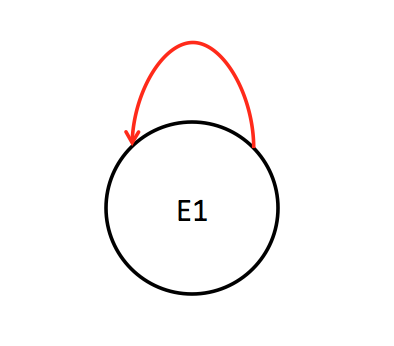
\includegraphics[scale=0.5]{selffeedback}
	\caption{\it Simple feedback loop with an entity supplying its input from its output.}
	\label{fig:exampleselffeedback}
\end{figure} 
Feedback loops can encompass multiple entities, in Fig.~\ref{fig:exampletwofeedback} a feedback loop is shown that encloses two different entities. An output from $E2$ is passed to $E3$ which in turn creates a new input for $E2$; though $E2$ input is not directly its own output, it does depend upon it. 
\begin{figure}[H]
	\centering
	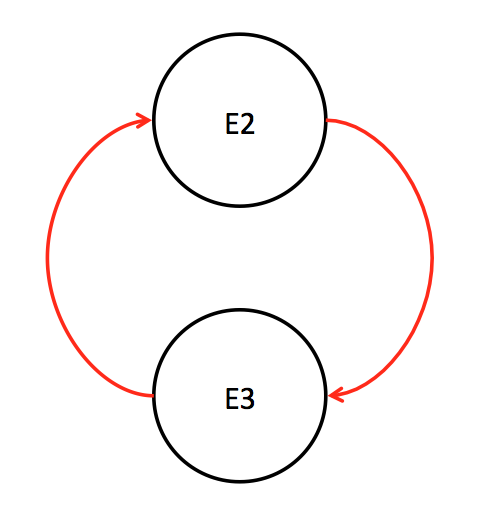
\includegraphics[scale=0.5]{twofeedback}
	\caption{\it Feedback loop between two entities, with each output being transformed by the other entity before becoming an input.}
	\label{fig:exampletwofeedback}
\end{figure} 
A loop such as the one in Fig.~\ref{fig:exampletwofeedback}, is only considered a feedback loop if information is passed through out the entire loop. If $E3$ produced a constant output, or an output that does not depend upon its input from $E2$, then this would not be a feedback loop as the new input to $E2$ does not depend on its output.

These examples are very simple, feedback loops can be much more complex, encompassing any number of entities, each of whom can have very complex algorithms for transforming their inputs. Feedback loops can operate across time, meaning that an event in the past can eventually feedback to a present decision. For a feedback loop containing a large number of entities the time scale on which the feedback occurs can be come significantly large.

Though feedback loops are often assumed to be a negative property, some can be stabilising due to a benign effect~\cite{beginref}.

Feedback loops can be present in a system in two ways, either they can be a constant fixture, called a static feedback loop, or they can form and change, called a dynamic feedback loop. A static feedback loop is present in the system from the start whether this is intentional and known, or unintentional and unknown to the members of the system. Dynamic feedback loops may not be present at the start and can form and change over time, with new entities joining or leaving them, allowing them to increase or decrease in size or effect, to split or merge, or to disappear.

Due to the potential complexity of feedback loops both in construction and in time, they can be difficult to detect, therefore methods are usually used to expose them. For static loops, forms of static analysis can be used such as analysing initial setup; this is possible since the loops do not change through out time. Dynamic loops can be much harder to observe and analyse, an important aspect to detecting these loops is the interactions, messages sent between different entities within the system. Since the loops can evolve over time being able to track and analyse these messages over a time series is vitally important for the analysis of these loops; this time dependent analyse is called dynamic analyse.

Since feedback loops can be destabilising and damaging to the system in which they occur, there is interest in studying this emergence in the aim to prevent monetary loss and damage to the economy.

Flash crashes are a notable form of emergence behaviour, due to feedback loops, that are considered damaging. These cause the price of a security or commodity to drop very rapidly, becoming disconnected from its fundamental, before then recovering~\cite{rareeventflashcrash}. A particularly famous flash crash is that of 2010, in which the E-mini S\&P 500 equity futures market dropped in price by more then 5\%, before rebounding to close to its original price~\cite{SECreport_delays, rareeventflashcrash}. This whole process occurred very rapidly, lasting approximately thirty-six minutes and has been described as``one of the most turbulent periods in their history'' for the US financial markets~\cite{Impact_hft}.

Research done by~\cite{DynamicCoupling_Chris, otherabmflash} describes how the crash may have unfolded due to a feedback loop between High-Frequency Traders (HFTs), known as ``hot-potato'' trading.

HFTs are a subset of algorithmic traders who normally participate in the market as arbitrageurs or market makers, they invest in ultra-high speed technology allowing them to detect, analyses and react to market condition in nanoseconds \cite{hftinformation1}. This means HFTs can trade huge quantities of assets in very short time frames, with some estimates stating that 10-40\% of all trades where initiated by them during 2016 \cite{hftmarketparticipation}.

The feedback loop of ``Hot Potato'' trading, is when inventory imbalance is repeatedly passed between HFT market makers. A market maker is a trader who is required to have both a bid and an ask on the order book at all times, this means in theory that they are constantly buying and selling. A high frequency market maker as expected should be buying and selling very very often. Market makers make a profit from the spread and not from long positions, hence they want to keep inventories low to avoid the market moving against them. To achieve this market makers have strict inventory limits that if they pass will cause them to sell off an amount of inventory to return back into their normal trading region. This inventory now sold by the market maker can be bought by another market maker perhaps causing them to exceed their limits and sell, this process is ``Hot Potato'' trading and can in theory be cyclic and continue indefinitely~\cite{Elias_Paper}.

This constant selling and buying of inventory can artificially inflate the trading volume of the market, changing how many traders operate and potentially leading to a flash crash.

Flash crashes have occurred on a number of occasions and in a large selection of markets, with a more recent example being a crash of the cryptocurrency Ethereum~\cite{cryptocrash}.


\subsection{Methods for Modelling Emergent Behaviour in Finance}  \label{litreviewofabmrr} 
There are many different methods available for modelling systems that may exhibit emergent behaviour, such as: 1-period, 2-period and multi-period models, probabilistic models (e.g. hidden Markov models), ordinary differential equations and partial differential equations~\cite{modles1, modles2, moldes3, moldes4}. This dissertation focusses on two models that can be used for discrete non-equilibrium system: recurrence relations and agent-based models. 

Both recurrence relations and agent-based models have been used in modelling the financial markets~\cite{rra10, rra1, abma2}.

Recurrence relations have seen wide spread use in economics appearing in a large selection of journals, including numerous times in top journals~\cite{rra2, rra3, rra4, rra5, rra6, rra7, rra8, rra9}. This wide spread use of the technique implies the acceptance of recurrence relations within financial modelling.      

Agent-based models are also used widely in economics and finance~\cite{abma3, abma4}. However these papers are noticeably absent from top economics journals (with some exceptions, such as~\cite{abmexp1} and~\cite{abmexp2}) and tend to be published in the Journal of Economic Behavior \& Organization and the Journal of Economic Development \& Control~\cite{whereabmp, farmerfoleynature}. The lack of agent-based models present in top economic journals combined with the number of papers published in other journals shows the lack of wide spread acceptance for this technique~\cite{agbntj, econmistsnoabm, lob_noecomimists}.

Here these two modelling techniques will be described.  


\subsubsection{Recurrence Relations} 
Wimp~\cite{recurrelationbook} describes recurrence relations as follows, recurrence relations connect a discrete set of elements in a sequence, these elements are normally either numbers or functions, they can be used to define these sequences or produce the elements in them. They can be seen as equations that give the next term in a sequence based on the previous term or terms, hence defining said sequence. Recurrence relations are often used to define coefficients in series expansions, moments of weight functions, and members of families of special functions.

The most simplistic form of a recurrence relation is one where the next term depends only on the immediately preceding term. If the $n^{th}$ element in the sequence is defined as  $x_{n}$, then this recurrence relation can be written as,    
\begin{equation}
x_{n+1} = f(x_{n}),
\end{equation}
where $f()$ is a function that calculates the next term based on the previous one. A recurrence relation does not just have to depend on its immediate previous term and can depend on any number of terms further back in the sequences. For example a recurrence relation depending on terms from two and three steps before can be written as, 
\begin{equation}
x_{n+1} = f(x_{n-1}, x_{n-2}),
\end{equation}
with $f()$ now taking two inputs to produce the new term in the sequence~\cite{recurrealtionwebpage}.

Recurrence relations can also be used to define a sequence through time. In the simplest case, the enumerate $n$ can be set to represent time $t$; this is applicable to discrete time as it requires set steps between the different times. Just as in the previous examples, the simplest recurrence relation is,  
\begin{equation}
x_{t+1} = f(x_{t}),
\end{equation}
where $x_{t}$ is the term at time $t$ and $f()$ gives the term at $t+1$ based on the term at $t$. Again this can be expanded to include terms from a number of previous time steps, allowing the memory of the sequence to be shown.
 
A recurrence relation for defining a sequence may also depending upon some parameter,  $\alpha$, in its simplest case this can be written as, 
\begin{equation}
x_{n+1} = f(x_{n}, \alpha).
\end{equation}
The next term in the sequence may not only depend on previous terms within its own sequence and parameters, it can also be conditional on another sequence. For example one sequence through out time, $x$, may depend on another sequence through out time, $y$, a simple recurrence relation for this could be,
\begin{equation}
x_{t+1} = f(x_{t}, y_{t}),
\end{equation}
with the sequence for $y$ possibly depending on its own recurrence relation. The sequence for $x$ may not even directly depend on its own sequence and could solely depend on $y$, 
\begin{equation}
x_{t+1} = f(y_{t}).
\end{equation}
Though it could also indirectly depend on its self, if $y$ was defined by a recurrence relation depending on $x$, such as, 
\begin{equation}
y_{t+1} = f(x_{t}).
\end{equation}
These cross sequence associations allow for complex interactions to be represented as time series defined by recurrence relations.

Recurrence relations have a number of benefits given by their construction, such as:
\begin{itemize}
    \item A mathematical formalisation of the whole system being modelled is given when using recurrence relations due to three factors: the way in which they model the whole system as an entity, the static view point they give to the system, and the mathematical stye which they take~\cite{rrformulism}.
    \item Links within sets of recurrence relations are hard coded into the equations, making these relationships amenable to static analysis.  
    \item This model lays out both the functionality of each equation and the relation between them in such a way to give a static representation of the system as a whole. 
\end{itemize}

A downside to this modelling technique comes with complex equations. Equations such as those making function calls within conditional statements, can be become increasingly less amenable to static analysis for dependencies. This is a problem similar to determining whether arguments will be evaluated, and makes tracking the flow of information, especially dynamically, very difficult~\cite{willevaluteargsa}. This also leads to challenges in in tracking the individual behaviour of recurrence relations or groups of recurrence relations~\cite{rrbtrack}.         







\subsubsection{Agent-Based Models}
A modelling technique that takes a more dynamic approach is agent-based modelling. Agent-based modelling can be considered more of a mind set than a rigid methodology; this involves describing the system in question in terms of its components and then allowing these to interact. Agent-based models allow a system to be described naturally and are hence the canonical approach to modelling emergent phenomena. This method is a bottom up approach, allowing for each component of the system, agent of the model, to be created to a relevant degree of abstraction~\cite{abmhumsystems}.

Agent-based models have been used to model a wide range of emergent behaviour including in the financial markets, examples of this are, noise traders~\cite{abmnoisetraders}, herding among traders~\cite{abmherding}, and fundamentalists~\cite{abmfundemetilists}.

Agent-based models are particularly suited to systems that, contain a number of autonomous components. Each component can be modelled independently and then allowed to interact through messages sent between each other. This allows for an obvious visual design of the system, such as that shown in Fig.~\ref{fig:abmii}.
\begin{figure}[H]
	\centering
	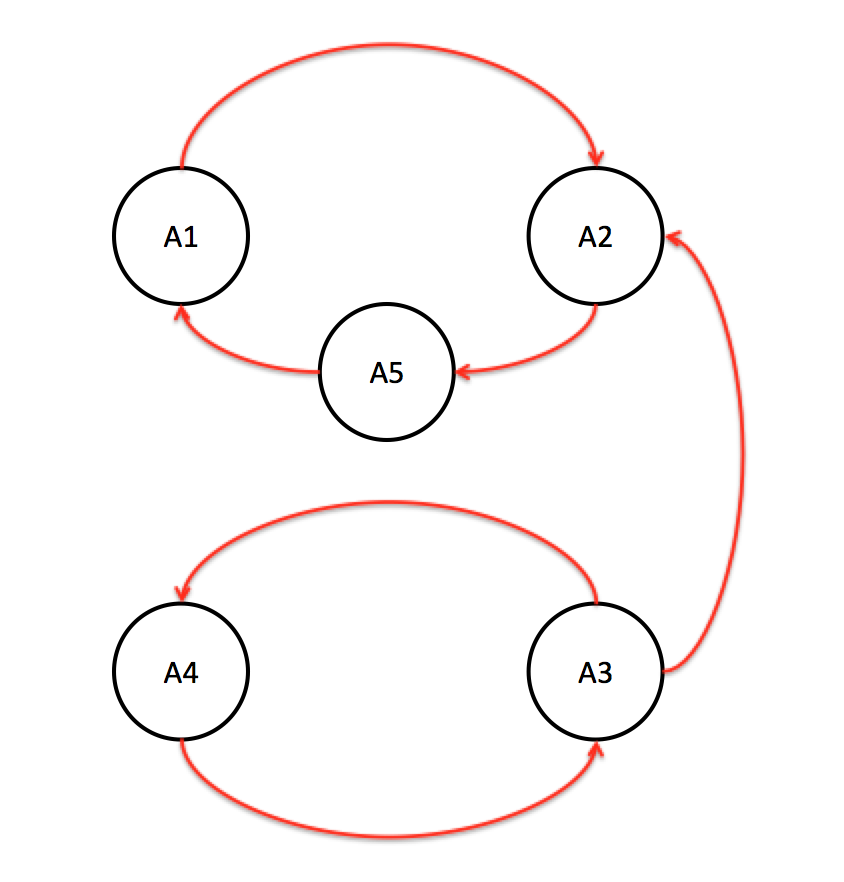
\includegraphics[scale=0.5]{abmii}
	\caption{\it Visualisation of the allowed interactions between five different agents, represented by black circles, with red lines representing the message paths.}
	\label{fig:abmii}
\end{figure} 
The main aspect of this model is the agents used. Though every system modelled can have drastically different agents, there are a few characteristics which should be in place for an agent to be considered an agent~\cite{MN2010, abmtsd}:
\begin{itemize}
   \item An agent is self contained, unique and identifiable, this requires an agent to have boundaries which can easily be used to determine what is and what is not part of the agent. 
   \item An agent is autonomous and it can act independently during its interactions with other agents. Its has behaviour and decisions that can be associated with information acquired  during communication with other agents. 
   \item An agent$'$s state varies over time, representing variables associated with its current position. 
   \item An agent$'$s behaviour is influenced by dynamic interactions with other agents. 
\end{itemize}

This modelling technique has a number of benefits originating from its construction, these include:
\begin{itemize}
   \item Being able to independently create each agent to varying degrees of complexity. 
   \item Giving a clear visual representation of the system$'$s interconnectedness.
   \item Giving a dynamic representation of the system.
   \item Easily expandable by adding more agents.  
\end{itemize} 

Since each agent in the system can be completely autonomous and independent from each other, save for message passing, this allows for them to be created individually. Hence each agent can describe its relevant component to a relevant degree of complexity, making the creation of a simulation more intuitive and sectioned. This makes agent-based models in many cases the most natural way for describing systems composed of ``behavioural'' entities~\cite{techsadsProbsabm}.

Due to the set up of this model a network representing the communication between different agents is easy to construct; this allows for topologies to be visualised and can aid in the creation of a simulation.    

The use of messages and a bottom-up approach in this model, allows for a more dynamic view of a system to be achieved; messages can be more easily tracked through-out the system$'$s evolution allowing for events to be more easily pinpointed and analysed.  

The use of independent agents makes this technique very amenable to expansion, new agents can often be added with little or no change to previously existing agents. This allows these simulations to be confidently expanded to look at more complex systems, or to add new elements to an existing system.  

These aspects of this approach make the modelling technique well qualified for modelling and analyse of emergent behaviour within systems of interacting components. However this approach does contain some draw backs including a one-to-many problem (where, though some high level behaviour may be noted in the system, this does not mean the only way of achieving this behaviour is the current system design) and the lack of a formal definition for the system as a whole~\cite{agbntj}.  



\subsection{InterDyne} \label{InterDyne_section}
An example of an agent-based model used in modelling the financial markets is InterDyne. InterDyne is bespoke simulator created by Clack and his research team at UCL~\cite{Chris_webPage}, it is a general-purpose simulator for exploring emergent behaviour and interaction dynamics within complex non-equilibrium systems.

InterDyne$'$s design is that of an agent-based model interacting via a harness. This creates a structure of individual autonomous agents who interact through messages sent through a harness to one another.
 
Similar to other agent-based models, InterDyne operates in discrete time rather then continuous time. These quantised time chunks, which move the simulation forward, can be left without proper definition (allowing operations to be defined in a number of time steps) or they can be equated to a real time (usually with the smallest time gap needed being a single time step and then all other timings being integer multiples of this). This discrete time is most important to message passing, with messages between agents only sent on an integer time step.

Messages in InterDyne are small packets of data, such as a series of numbers. An agent can send private messages that are only received by a single other agent (one-to-one messages), or it can send public broadcast messages received by any number of other agents, subscribed to a channel (one-to-many messages). To facilitate this a communication topology can be made for InterDyne, this is done in the form of a directed graph determining which agents can communicate with each other. Due to the directional nature of these messages this topology could allow an agent to send messages to another but not be able to receive messages from that same agent. Messages have a defined order to them, an agent will, unless otherwise instructed, always process messages in the order in which they arrive. To change the order in which messages arrive delays can be added to communication paths between agents, this can be a static delay which always applies to messages sent from one agent to another, meaning this will arrive a set number of time steps later. Or a more complex dynamic delay, which is achieved by using another agent to mediate the passing of these messages, delaying by an amount decided on in some internal logic. All messages in InterDyne are passed through a harness; this does not alter the messages or delay them,\footnote{Unless instructed to, using a static delay.} but does store the messages and their order which can be used in post analyse.
        
Each of the agents within an InterDyne simulation can be completely unique and modelled to different levels of complexity, as is the case with most agent-based models. As a whole InterDyne simulations are deterministic, repeated experiments will return identical results. However non-determinism can be added via the agents, making some part of an agent stochastic, and will lead to repeated experiments on the whole returning different results. A pseudo-random element can also be added by instructing InterDyne to randomly sort the message order for any agent receiving multiple messages in one time step. This is only pseudo-random as, as long as the same seed is used each run of the simulation will order the rearranged messages in the same way.\footnote{If an agent receives multiple messages at the same time step and the pseudo-random element is not being used, these messages will order based on the identifiers of their sender agents.}

InterDyne is created to be particularly amenable to dynamic analyses of its simulations, this is achieved in part by all messages being sent via the harness allowing them to be recorded for post processing.     


\subsubsection{Applicability to Finance} \label{applicabilut_to_finance}
InterDyne has been designed with modelling flash crashes in the financial markets in mind and has a number of features that make it well suited to this purpose. 

\paragraph{Deterministic}
The deterministic nature of InterDyne allows for experiments to be run multiple times with the same result always returned, this allows for changes to the experiment setup to be investigated. For example changing the number of traders in the market and comparing this to a previous run allows for an investigation into how many traders are required for emergent behaviour to be observed.

This becomes particularly interesting when comparing the interactions between market makers to that of the n-body problem. Like with this problem one could expect emergent behaviour might occur to some extent in a large group of market makers, however the question of whether emergence persists in a comparable market to the three-body problem and how this compares to a larger market can be investigated.   

\paragraph{Message Delays}
Allowing for messages to be delayed is needed to facilitate hypotheses involving delays as a factor for emergent behaviour. Delays have been suggested to have caused ``hot potato'' trading during a flash crash, these delays can exist due to processing time and transmission time of messages~\cite{SECreport_delays}.

InterDyne allows for both symmetric and asymmetric, delays. These delays can be static or dynamic, with dynamic delays requiring a special intermediary agent. 

\paragraph{Storing Messages}
InterDyne facilitates analyses of simulations by allowing for the messages between agents to be stored and viewed as a trace file. This can include all messages as well as timings, and messages can also be sent directly to the harness which will be added to the trace file. 
  
\paragraph{Message Ordering}
The order in which messages are processed can be very important. For example in an exchange, it can change whose limit order has priority at a given price and whose market order executes the lowest prices. Changing these factors can make or break feedback loops within the system, meaning if message ordering is not properly dealt with the correct emergent behaviour may not be observed. Hence InterDyne stores messages in the order they are received by an agent, taking into account delays to the messages. This however can not be done when multiple messages are received at the same time step, due to the nature of discrete time there is no way for the agents to know which message arrived first. Therefore two options are presented by InterDyne; messages are ordered according to their agent identifier or messages are randomised and executed in the emerging order.



\subsubsection{InterDyne Detailed Operation}
InterDyne is written in the functional language Haskell. The structure of an InterDyne model is show in Fig.~\ref{fig:harness_setupfigure}, this structure contains a number of agents and a simulator harness. These agents send two types of messages, either one-to-one or one-to-many (broadcast) messages. Both these messages are sent to the harness, the harness then resends these messages to the appropriate agents, one-to-one messages are sent to their target agent and one-to-many messages are sent to any agent subscribed to the relevant broadcast channel. Messages can also be sent directly to the harness and not rerouted to another agent. At the end of the simulation the harness will produce a trace file containing information on all the messages sent for post-hoc analysis.    
\begin{figure}[H]
	\centering
	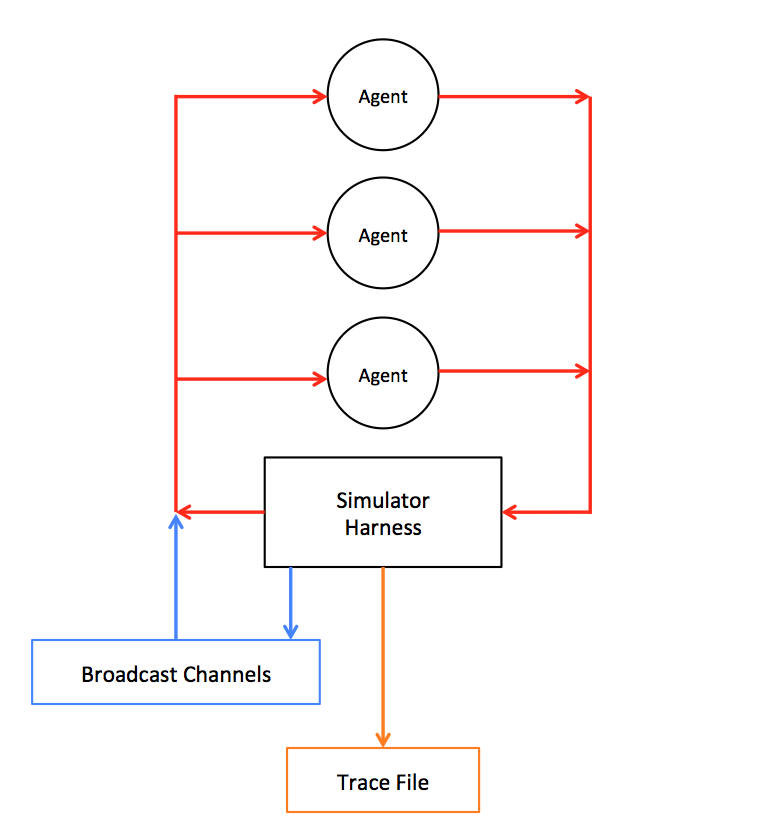
\includegraphics[scale=0.5]{harness_setup}
	\caption{\it Structure of an InterDyne simulation containing three agents. The messages sent by the agents to the harness and from the harness are coloured red. The trace file and messages sent to the trace file are coloured orange. The messages sent from the harness to the broadcast channels and then back to the agents are coloured blue~\cite{interdynemanual}.}
	\label{fig:harness_setupfigure}
\end{figure} 
%-topology and delays 
InterDyne has an intrinsic delay, which means any message sent will not be received until the next time step; message sent at $t$ will be received the earliest at $t+1$. This is in part due to the fact that the harness compiles all messages from a single time step before sending them to their targets and hence initiating the next time step. The harness can be seen as the driver in the simulation sending out the message and forcing the agents to send their next message.   

Longer delays can also be added using InterDynes topology, this allows for any two agents to be selected (a sender and a receiver) and for a delay between them to be given. This topology takes the form of a directed graph, with the agents acting as the nodes and the interaction routes as the links, this allows for the delays to be asymmetrical. Using this, a delay for a path could also be set as an abort message, making a particular communication route unusable.  

Adding delays is done through run time arguments, here two run time arguments must be added, one stating the maximum delay in the system and the other listing the delays. To show the maximum delay the argument $(Arg (Str$  $``maxDelay", 10)))$ is used, where $10$ is the maximum delay. To add the list of delays the argument $(DelayArg (Str$  $``DelayArg", delay))$ is used, where $delay$ is a function that takes two agents and returns the delay between the first and the second. 
%-what a message looks like 

Messages sent between agents can in theory be as complex as needed, these messages do however have to comprise of the following components: 
\begin{itemize}
   \item A tag indicating the type of message being sent, e.g. a broadcast message.
   \item A tuple of two integers, with the first being the sending agents ID and the second being either the receiving agents ID or the receiving broadcast channels ID.  
   \item The data that is being sent. 
\end{itemize}
An example of this is a one-to-one message, for example $Message$ $(1, 2)$ $data$, where $data$ is the information being sent from agent $1$ to agent $2$ 

A broadcast message, for example $Broadcastmessage$ $(3, 1)$ $broadcastdata$, can be received by agents subscribed to its channel, in this case $1$. All agent subscriptions to broadcast channels have to be announced at the beginning of a simulation and can not be changed during it. This is done by adding the subscription channel to the list in a tuple passed as an argument, for example this could look like $(agent1, [1])$, for agent 1 subscribed to broadcast channel one.

Empty messages can also be sent, if the message is required to be known to be intentionally empty and not a mistake, the a message can be sent containing ``Hiaton''. This is done at the beginning of the run to allow for the harness to send a first message. 
%-what is an agent in interdyne and what is its type

InterDyne is designed in such a way that agents both take in and produce a seemingly infinite list of messages. This is achieved through lazy evaluation in Haskell, which in short means that any element in the list will not be calculated until it is absolutely needed. This allows for an infinite list as long as no agent tries to read further into the list than what has already been calculated. In achieving this an agent must at each time step, read in a message (even if it is then not used) and produce a list of messages (even if this is an empty list). An agent will hence iterate over the list of incoming messages, at each time step adding a new output message to its list of output messages.  

Agents in InterDyne are typically, though not required to be, written in two parts, a wrapper function and a logic function. The wrapper will manage the reading of inbound messages to the agent and generate its outbound messages, it will also update the local state of the agent. While a logic function is called by the wrapper to calculate the messages to be sent and their content. An agent written following this design could have a form similar to that of the agent show in Fig.~\ref{fig:wrapperfrominterdyne}. This agent$'$s wrapper recursively calls itself on the inbound message list, consuming the head of the list\footnote{This design dictates that the head of the list is the messages for the current time step.} and producing a list of outbound messages using a logic function.  
\begin{figure}[H]
	\centering
        \lstinputlisting[language=Haskell]{complexagentwrapper.hs}
	\caption{\it Simple wrapper function, which creates a list of output messages by iterating through a list of inbound messages and calling the sub-function $logic$.}
	\label{fig:wrapperfrominterdyne}
\end{figure} 
%-what is the harness in interdyne and what is its type

The simulator harness is an intrinsic part of the simulator, it drives the simulation, handles message passing and produces the output trace file.

This has the type shown in Fig.~\ref{fig:harntypintfirst}, this type illustrates the functions input of a number of steps and runtime arguments (with agents and the broadcast channels they are subscribed to). The output from this function can be seen to be of type $IO()$, this is writing the trace information to file.  
\begin{figure}[H]
	\centering
        \lstinputlisting[language=Haskell]{harntypint.m}
	\caption{\it Type definition of the function sim.}
	\label{fig:harntypintfirst}
\end{figure} 


The simulator harness is embodied in a function called sim, this function contains code associated with a number of administrative operations. For the purpose of this project a reduced specification of the function sim will be shown. This specification captures all of the core functionality for managing message passing for agents and driving evaluation of the simulation. This reduced InterDyne sim harness can be seen in Fig.~\ref{fig:intersimfun}, with its function type shown in Fig.~\ref{fig:reducedsimtypet}. This reduced function is shown outputting a single integer value, that is the first message sent by the first agent at time step $x$. This is just for illustration purposes since the normal output of sim is a trace file and is not being shown here. In the reduced type definition it can be seen that the output is now and integer instead of an $IO()$ type, the list passed to the sim that contains the subscription channels is now of unknown type as no channels are passed.   
 
\begin{figure}[H]
	\centering
        \lstinputlisting[language=Haskell]{intersimfun.hs}
	\caption{\it Reduced InterDyne simulator. This sim function outputs, the value of the first messages from the first agent at the final time step.}
	\label{fig:intersimfun}
\end{figure} 

\begin{figure}[H]
	\centering
        \lstinputlisting[language=Haskell]{harntyptrans.m}
	\caption{\it Type definition of the reduced function sim.}
	\label{fig:reducedsimtypet}
\end{figure} 

%-how do you run an interdyne experiment 

%Running an InterDyne experiment is done by calling the simulator with relevant inputs, an example example of this is shown in Fig.~\ref{fig:runninginterdyne}.
%\begin{figure}[H]
%	\centering
%        \lstinputlisting[language=Haskell]{interdynewithdelays.hs}
%	\caption{\it A run of an experiment in InterDyne containing delays.}
%	\label{fig:runninginterdyne}
%\end{figure} 








\newpage
\section {Description and Analysis of the Problem} \label{despriptionandanalysproblem}

Investigating emergent behaviour originating from interaction dynamics, within a complex system, relies on viewing the communication between different components of the system as messages being passed. These messages can then be analysed to assess the communication and its pattern that lead to the creation of the emergent behaviour, this approach is amenable to the discovery of phenomena, such as dynamic feedback loops. A model investigating emergent behaviour hence must be able to view communication as messages being passed between different components. For results from this model to be broadly accepted, in fields such as economics, the model as a whole must also be well defined.      

Agent-based models naturally support a message passing view making them well suited to analysing and investigating emergent behaviour. However most agent-based models, though having each individual agent fully specified, do not have a well defined formalisation for the system as a whole. This makes it challenging to perform system wide analytics on most agent-based model. Recurrence relations naturally support a system wide analysis, due to the full definition of their models. However their formulation does not support a message passing view of communication between components, making it difficult to analyse emergent behaviour with them directly. 

This creates a problem as neither model is perfect for the task at hand. A resolution to this problem suggested by~\cite{econmistsnoabm}, is to give a formal definition of the specification of an agent-based model as a set of recurrence relations. 

This section discusses how relating these two models can be achieved, reviews literature on work done formalising agent-based models, and discusses challenges related to the method presented in this dissertation.  


\subsection{Method for Achieving a Translation}
%%%%%%How can this solution be achieved (translation form rr to abm)
To allow for recurrence relations to be used in formalising an agent-based model, the two paradigms must be connected. This connection must be able to demonstrate some sort of equivalence between these two models. 

It has been shown informally by~\cite{gabm3} that most agent-based models can be expressed as a set of partial recursive functions. Therefore it can be inferred that a connection between a recurrence relation model and an agent-based model can be created in the form of a translation, from one to the other. 

%%%%%%what is a translation between rr and abm
A correctness preserving translation between a recurrence relation model of a system and a agent-based model of the same system; allows for the recurrence relation model to provide a formalism for the agent-based model. Correctness preserving in this context is used to mean that both models representing an identical model and will produce identical results; so that both views of the system should be completely interchangeable. 

%%%%%%what direction should this translation take and why? rr -> abm
An important consideration in creating a translation between the two methods is, which direction this translation should take. For the purpose of defining the formalisation of an agent-based model and hence increasing its acceptance for a reader, a recurrence relations to agent-based model trajectory is preferred. This ordering will allow a read to start with a formalised description and translate this formalisation to cover an agent-based model, as opposed to starting with an unformalised model and translating to a formalised one. This process essentially creates and agent-based model view of the recurrence relation model.      

%%%%%%How will this translation be done? look at work other people have done on translations (step-by-step) 
The next consideration is how this translation will be achieved. Inspiration can be drawn from other works investigating the design of translations, such as~\cite{clovertrans},  \cite{transproggotmod} and  \cite{stepcorentconv}. These three papers discuss translations between program representations in a way in which, the final representation will faithfully represent the initial. The approach taken by these papers is to increment the translation in step-by-step manner, where each step slightly transforms the previous to be closer to the final form. The benefit of this method is that if each step on the translation can be proven to be correct then the whole translation can be seen as correct. This approach relies on the correctness of the steps being transitive; that a correctness preserving translation from state 1 to state 2, and then another from state 2 to state 3, will produce a correctness preserving translation from state 1 to state 3.\footnote{A formal proof for a correctness preserving translation will be discussed in Section~\ref{furtherwork}.} 

%%%%%%what is the project? (make rr language, convert in a step-by-step manner to InterDyne
A connection between these two models can hence be created by translating in a step-by-step fashion from a recurrence relation language to an agent-based model. The agent-based model used in this translation is InterDyne and the recurrence relation language used is discussed in Section~\ref{beskoperecurrancerealtion}. InterDyne was selected due to a number of factors, most importantly InterDyne was designed from the bottom up to model and investigate emergent behaviour with the financial markets, with research already being conducted using it to this end~\cite{DynamicCoupling_Chris}, this software was also a convenient choice due to access to the source code and local expertise.

\subsection{Review of Similar Work}\label{simwork}
The idea of using recurrence relations to give a formal definition to an agent-based model is not a novel one and falls under the general heading of using formal systems to prove properties of agent-based models. Work in this area has covered game theory, discrete systems, classifier agents and equation-based models~\cite{taabm}. The use of recurrence relations falls under the classification of an equation-based model, these have been used in a number of papers looking to give a formalisation to agent-based models. Here three papers~\cite{ebmabmi}, \cite{econmistsnoabm} and \cite{abmtsd}, looking at this area will be reviewed and discussed, along with DEVS formalism introduced in Ref.~\cite{introdevs}.

Before reviewing these papers, it is worth considering the more obvious question of does a formalism need to be given by another modelling technique to allow for the analyses of an agent-based model? North~\cite{taabm} present$'$s a formalism for the analysis of agent-based models, looking in particular at performance. This paper looks to prove findings from agent-based models, in particular the focus is on existing agent-based software such as Swarm, Repast 3 and others. This paper notes that these pieces of software use a modular imperative architecture with factored agents, spaces, a scheduler, logs, and an interface. Hence this paper presents a theoretical formalism for analysing a modular imperative agent-based model.    

This formalism is presented using an abstract machine specification of the modular imperative agent-based modelling architecture. A  Random Access Stored-Program (RASP) architecture was chosen for the abstract machine, this architecture had been created in an earlier paper~\cite{raspceated} and was chosen due to its similarities to real computer systems. This is opposed to other options including Turing machines and $\lambda$-calculus, as they are less well matched with modern computer systems.     

One of North$'$s motivations for using this technique over an equation-based model formalisation, is that he claims that a formulation of the agent-based model in terms of an equation-based model would be unnatural and possibly unrecognisable to those accustomed to agent-based models. This consideration is not as important to the work presented in this dissertation, since here the aim is to familiarise those accustomed with equation-based models to agent-based models and not the reverse. The same argument applies to the use of RASP over alternatives such as $\lambda$-calculus, this dissertation is more interested in creating a formalism which is relatable to economists over computer scientists.   

In~\cite{ebmabmi} Costa et al consider the formalisation of agent-based models by creating their implementation guided by equation-based models. an (equation-based model)-oriented design. This paper looks at an example with interacting entities with given strategies, however these strategies could change upon interactions. In this example the equation-based model took a probabilist and macro-view approach where the agent-based model, due to its nature, took a micro-view approach. The analyses of these two models showed that though the systems appeared to be the same the micro-view approach could create slightly different outcomes depending on the number of agents chosen. This difference comes from the fact that the individual agents in the agent-based model were created to match a macro-level description given by the equation-based model, however due to the autonomous nature of the agents only their general behaviour can match and in certain circumstances even this did not correctly produce the behaviour. This issue spawns from trying  to recreate the behaviour of a probabilistic model using a deterministic model. 

This paper concludes summarising the benefits of this approach in validating an agent-based model, here an agent-based model is known to be a faithful representation of the system as long as the equation-based model is a faithful representation. However the question of whether the agent-based model is correctly implemented still rests with that model. 

The main difficulties faced by this paper appear to be the transformation from a macro-level view (equation-based model) to a micro-level (agent-based model) view, this is particularly due to the statistical nature of the equation-based model. Though they succeeded in creating a formalisation of their model the differences in results between runs still raises questions over the equality between the two view points. To avoid this issue, a more micro-level focussed equation-based model should be taken.

The next paper is~\cite{econmistsnoabm}, this paper is based on a similar principle to this project in that it seeks to bridge the conceptual gap around  agent-based models in economics. It tackles this problem by introducing an equation-based formalism to describe both agent-based models and analytical models, though of interest here is their work on former. 

The agent-based model is formalised by specifying how each agent\textsc{\char13}s state within the model changes between each time step. This is done by defining agent attributes using vectors of state variables and then applying time-indexed difference equations to specify each agents state change. This allows for expression of the agent-based model in terms of difference equations, which they then use to look at parameter estimation. 

Their work shows the ability to provide estimations on agent-based models, counter to some criticism that has been levelled at agent-based models. Some difficulty in this approach can come from agent-based models with complicated algorithmic behaviour within the agents, specifying these models as difference equations can be challenging task. The work in this dissertation does not directly suffer from this problem as all systems are first described as recurrence relations before being translated into agent-based models, meaning that the equation view will only be as complex as the original writer intends.  

Macal~\cite{abmtsd} investigates relating Forrester\textsc{\char13}s System Dynamics (SD) model to an agent-based model. System dynamics models consist of a set of difference equations, so this can be seen as a comparison between difference equations and agent-based models. This paper presents a formal specifications for both the Forrester\textsc{\char13}s and agent-based models, these specifications are then compared to show their equivalence. Once equivalence has been proven the specification of a Forrester\textsc{\char13}s model can be used to derive an agent-based model that is an correct representation of the same system.

This technique is applied to an SIR epidemic model, creating a Forrester\textsc{\char13}s and agent-based model representation. These two descriptions of the system are then evaluated and have their results compared. The findings show that though both models show similar behaviour, there is not an exact match between them. This is due to the probabilistic nature of the system being modelled and the different approach that an agent-based model takes to these kind of systems. 

This paper, though showing equivalence, does so in a more abstract manner then a direct translation between the two models. The difference in experimental results from the two models is down to the use of describing the system in a probabilist fashion, this can be avoided by describing a system in a more micro-level view.    

A discussion relating to the formalism of agent-based models would be amiss without mentioning the Discrete Event System Specification (DEVS)~\cite{introdevs}. DEVS is a theoretical formalism designed for analysing complicated simulations, which it does by describing simulations as hierarchical Moore machines, with additional timing information added to the state transitions. DEVS has a few variants including classic DEVS (this is the core abstraction), coupled DEVS (allows for hierarchical nesting of the Moore machines~\cite{coupleddevs}) and Dynamic Structuring DEVS (attempts to allow for dynamic behaviour~\cite{dynamicdevs}).

DEVS is able to provide a theoretical foundation for analyses of a number of critical computational properties of agent-based models, including properties such as decidability. In theory DEVS has the ability to represent any computational model, including agent-based models. However though DEVS is capable of representing an agent-based model it is not necessarily the best approach. Despite the work done in~\cite{dynamicdevs}, DEVS is still not an ideal match for models that have dynamic behaviour, such as agent-based models where agent behaviour can be dynamically generated. Classic DEVS imposes boundaries between states and behaviours making dynamic behaviour difficult to represent, where as Dynamic Structuring DEVS introduces new constraints that have a similar effect in limiting utility. These constraints and difficulties make it challenging to use DEVS as a formal basis for agent-based modelling~\cite{taabm}.  






\subsection{Challenges with the Translation Approach} \label{twoviewsapproach} 
The approach taken in this project of creating a step-by-step translation between a recurrence relation description of a system to a agent-based model description on the same system has a number of challenges associated with it. In this section the difficulties with this project will be described. 

As noted in Section~\ref{simwork}, when looking at work done by other researchers in this area, a main challenge was how to model systems that have no counterpart in an agent-based model. This problem exists mostly due to modelling probabilist systems and macro-level systems, which are counter to the view an agent-based model takes. In this project however the focus will be on systems which are modelled at the micro-level and without probabilist aspects, though stochastic aspects will be allowed within the micro-level view.

A problem overshadowing most aspects of this project is that the two paradigms being translated between are completely different and in some ways opposing. Recurrence relation models take an analytic (where the system evolution is defined statically.) approach where as agent-based models take a dynamic one (where the system evolution is given in simulation).  %is this right (help) 

The formulation of how information is exchanged within these two models is also in contrast. Recurrence relations take a static view with information passed via function calls, opposed to the agent-based model approach of dynamically sending the information between agents using message passing. This represents a difference in the way information is seen in these models, in recurrence relations information is freely available and the equation wishing to use it simply has to make a function call. Where as in agent-based modelling information is given by its creator to only other agents selected by its creator, hence agents can not use information which has not been already sent to them.

The agent-based model selected for use, InterDyne, operates by making every agent take in an infinite list of their inputs and output an infinite list of their outputs. Creating this view of the system from a recurrence relation model, which is created as a snapshot of a current time step, is challenging. 

In InterDyne both direct and broadcast messages exist, these two messaging types can be seen as the use of private and public date respectively. Recurrence relations do not have an inbuilt method of distinguishing between different types of data as all information is passed by direct function calls, reconciling these two view points creates another challenge. 

In recurrence relations information from any previous time step can be easily accessed, whereas in InterDyne information is only available for the time step at which it was received. This creates the idea of time-limited information with InterDyne that is not present within a recurrence relations model.   

Agent-based models have name control, indicating the different agents and functions within them. However introducing name control to  recurrence relations, that have no sense of agents, in a way in which it is tangible to the agent-based model is a challenge. 

Recurrence relations access information directly as a value where needed; agent-based models however receive special item called a message that contains this value along with other information (e.g. the senders id). Translating between these two different ways of viewing values poses difficulties.  

There has been criticism that agent-based models splinter a model, finding a way to split the recurrence relations into agents with out splintering the model creates another challenge. 

The approach taken in this dissertation is to create a series of small steps between a recurrence relation model and an agent-based model, the smaller the steps are the easier it is for a reader to follow the process. However a challenge is finding how to create these small steps as it may often be easier to create large but less comprehensible steps.   








\newpage
\section{Bespoke Recurrence Relation Language} \label{beskoperecurrancerealtion}
This section introduces a bespoke recurrence relation model, created to be able to model complex systems with interacting elements. This recurrence relation model will eventually be translated into an agent-based model and hence needs to be able to express the system being modelled both statically and dynamically. 

A bespoke recurrence relation language is created for a few reasons: firstly there needs to exist a strict set of known rules to facilitate parsing of the language if the process is automated. Secondly, the functionality of the language needs to be restricted to keep it as simple as possible, to allow for the language to be readily understandable and easy to parse, only introducing complexity where necessary. Thirdly, the language still needs to maintain sufficient functionality to model complex systems. Creating a bespoke language offers a straightforward method satisfying these three criteria.     
 
A set of recurrence relation can be used to statically model a interacting system, however this model does not give a time dependent  experiment required for dynamic modelling. To add time dynamics to this model the set of recurrence relation described need to be traced through time.

To allow for tracing, specifications need to be give of a set of recurrence relations, initial values for these relations, and a driving expression. 

This section first gives the concrete syntax, then keywords and naming conventions, finally a well formed program in this language is described and an example is given.  
 


\subsection{Syntax}
The formal concrete syntax for this bespoke recurrence relation language is defined in Backus-Naur form (BNF), shown in Fig.~\ref{fig:bnflex}. The main aspects of this notation, in this context, are described as follows:
\begin{itemize}
  \item Expressions of the design of language are represented inside $<$ $>$; these are high level design aspects of the language (e.g. the simulation as a whole, or the main block defining the experiment).
  \item These high level expressions are given meaning by $::=$, the expression of the left hand side of this must take the form given on the right hand side (e.g. in $<a> ::= <b>$, $<a>$ has to take the form given by $<b>$).  
  \item The right hand side of $::=$, have multiple options, these are split by $|$. This can be seen to representing an $or$ operation, with the left hand side being able to be represented by any of the options given on the right hand side (e.g. in $<a> ::= <b> | <c>$, $<a>$ can be either $<b>$ or $<c>$). 
  \item The speech marks $``$'' are used to denote actual writing in the language, this allows the syntax to describe how the language can be written (e.g. connecting the expression $<where>$ to the word $``where$'' in the language). In this notation $``$'' are used for strings of characters, and $`$' are used for single characters (e.g. $``where$'' and $`w$').
  \item Here $..$ is used to denote any item that would logically appear between the left hand side and right hand side of the $..$, these items are separated by an $|$ (e.g. $`1$'$.. `4$' gives $`1$' $| `2$' $| `3$' $| `4$'). 
  \item The character $`\backslash n$' is used to donate  a new line in the language. 
\end{itemize}
\begin{figure}[H]
	\centering
	\lstinputlisting[language=Miranda]{bnflex.m}
	\caption{\it Concrete BNF syntax for the bespoke recurrence relation language.}
	\label{fig:bnflex}
\end{figure} 

A simulation written in this language takes the structure shown in Fig.~\ref{fig:befroemira}, this structure is defined to have the same meaning as the Miranda expression shown in Fig.~\ref{fig:miramean}; where the BNF syntax for the items encapsulated by $<>$ is shown in Fig.~\ref{fig:structuredefs}.

\begin{figure}[H]
	\centering
	\lstinputlisting[language=Miranda]{befroemira.m}
	\caption{\it Layout of a simulation in bespoke recurrence relation language.}
	\label{fig:befroemira}
\end{figure} 

\begin{figure}[H]
	\centering
	\lstinputlisting[language=Miranda]{miramean.m}
	\caption{\it Miranda definition of the layout shown in Fig.\ref{fig:befroemira}.}
	\label{fig:miramean}
\end{figure} 

\begin{figure}[H]
	\centering
	\lstinputlisting[language=Miranda]{structuredefs.m}
	\caption{\it BNF syntax for items shown in Fig.~\ref{fig:befroemira}, with further definitions defined in Fig.~\ref{fig:bnflex}.}
	\label{fig:structuredefs}
\end{figure} 

The syntax given in this section dictates how a simulation written in this bespoke recurrence relation must be formatted and what items are allowed to be used within this language. The functionality of this language, given by the BNF, will be described more fully in the Section~\ref{nameconv}. Any program that does not fit the shape described by the concrete BNF can not be considered to be a model written in the language defined in this section.  



\subsection{Naming Conventions} \label{nameconv}
This language has a strict naming convention, as well as some restricted names. Naming conventions are in place for recurrence relation definitions, where blocks, sub-functions, variables, initial conditions and  if statements. 

A recurrence relation be defined in four parts, $name$ $arguments$ $=$ $expression$. The name must be formatted in the manner $group\_name$, where $group$ is the name of the group the recurrence relation belongs to and $name$ is the name of the particular recurrence relation. Multiple recurrence relations can belong to the same group, and hence have the same group name, however only one relation in each group can have a set name. This language requires that all recurrence relations take at least one argument, and that time $t$ has to be the first argument. Time $t$ does not need to be utilised within the relation but it must be in the definition.     

A recurrence relation can have sub definitions relating to it, this is done through the use of a where block. A where block is written after the expression for a recurrence relation and starts with the keyword $where$. After this local definitions for internal functions and variables can be defined. 

Internal functions must be formatted in the manner $\_name$, where $name$ is the name for the function. These functions can only be accessed by the recurrence relation they are within. Local variables can be defined using the formate $name$, this name can be anything as long as it does not clash with restricted names or other variable names with in the where block. 

The driving expression is given in a defined section of the model, showing in Section~\ref{wellformedprogs}, and is written as  $group\_name$ $arguments$. The  $group\_name$ must correspond to a recurrence relation listed in the model and the $arguments$ must be given as values, allowing the recurrence relation to be evaluated. 

Initial conditions are listed in a special location in the layout, which will be show in Section~\ref{wellformedprogs}, and are defined in three parts $name$ $=$ $expression$. This name can be seen as a variable and can be anything not in the restricted name list. 

This language allows for both $arguments$ and $expressions$ to be written using: lists, numbers, variable names, recurrence relation names, internal function names, mathematical operators, brackets, some inbuilt functions, and conditional statements. 

List in this language are contained within $[]$, items within these lists are then separated using $,$.  

This language allows the use of both integers and decimal numbers, with $.$ used in decimalisation. 

Variables that have been defined and are in scope can be called by simply calling their name. 

Recurrence relations that are in scope can be called by calling their name with a relevant set of arguments.  

Internal functions that are in scope can be called by calling their name and a relevant set of arguments, if applicable. 

This language allows for the mathematical operates shown in Fig.~\ref{fig:bnflex}.

Expression can be incased in brackets by using $()$.

This language allows for the use of three inbuilt functions: $hd$ (returns the head of a list), $tl$ (returns the tail of the list), and $:$ (adds an item as the new head of a list).  

Conditional statements with in this language are written as $cond$ $condition$ $expression$ $expression$. Where if the condition is true, then the first expression is run and if not the second expression is.  

There are a number of names and naming conventions which can not be used and can be seen as restricted, these are:
\begin{itemize}
  \item The use of $\_$, unless it is being used for its designated purpose in recurrence relations and internal functions. 
  \item The use of the name $main$.
  \item The use of the name $init$.
  \item The use of the name $where$, unless used to make a where statement.
  \item The use of symbols, unless for their mathematical purpose.  
\end{itemize}






\subsection{Well Formed Programs} \label{wellformedprogs} 
This language has a strict style and layout, this covers a number of aspects: layout, experiment, initial conditions and recurrence relations.  

The layout of an simulation should match that shown in Fig.~\ref{fig:1exofla}, with $main$ signifying the experiment, $init$ the initial conditions and $where$ the list of recurrence relations. 

\begin{figure}[H]
	\centering
	\lstinputlisting[language=Miranda]{1layout.m}
	\caption{\it Layout of a simulation.}
	\label{fig:1exofla}
\end{figure} 

An experiment is written as a function call, with a certain set of arguments. Figure~\ref{fig:2exofla} shows a experiment that will return the value of the recurrence relation $i\_f1$ at time $3$.
\begin{figure}[H]
	\centering
	\lstinputlisting[language=Miranda]{2experment.m}
	\caption{\it Function call for value at time 3 in recurrence relation 1\_f1.}
	\label{fig:2exofla}
\end{figure} 
 
The initial conditions, which use will be shown later, are defined as shown in Fig.~\ref{fig:3exofla}. There is no defined  limit to the amount of initial conditions that can be defined. 
\begin{figure}[H]
	\centering
	\lstinputlisting[language=Miranda]{3initcons.m}
	\caption{\it Definition of two initial conditions, q and k.}
	\label{fig:3exofla}
\end{figure} 
 
A simple recurrence relation can be written as shown in Fig.~\ref{fig:4exofla}, this recurrence relation belongs to group $i$, is named $f1$ and takes one argument which is time $t$. The expression of this relation is to call itself at the previous time step and to add that to a call for another recurrence relation, from group $j$, at the previous time step. 
\begin{figure}[H]
	\centering
	\lstinputlisting[language=Miranda]{4rrsim.m}
	\caption{\it A simple recurrence relation, belonging to group i that adds its value at the previous time step to that of j\_f1 at the previous time step.}
	\label{fig:4exofla}
\end{figure} 
 
Initial conditions can added to recurrence relations using pattern matching, as shown in Fig.~\ref{fig:5exofla}. The recurrence relation is first written with the value for which the initial condition will be sent and this is sent to equal the initial condition, then the full recurrence relation is written.  
\begin{figure}[H]
	\centering
	\lstinputlisting[language=Miranda]{5rrint.m}
	\caption{\it Recurrence relation containing pattern matching for initial conditions.}
	\label{fig:5exofla}
\end{figure} 
 
An if statement, shown in Fig.~\ref{fig:6exofla}, can contain very complex components it is hence good practice to encase each expression with in a set of brackets to maintain legibility and correct functionality.  
\begin{figure}[H]
	\centering
	\lstinputlisting[language=Miranda]{6rrif.m}
	\caption{\it Recurrence relation using an if statement.}
	\label{fig:6exofla}
\end{figure} 
 
A where statement is used to provided additional functionality to a recurrence relation and can be used to make a expression more legible and help reduce human errors. Figure~\ref{fig:7exofla} shows the use of a where statement to add an internal variable and an internal function to a recurrence relation. 
\begin{figure}[H]
	\centering
	\lstinputlisting[language=Miranda]{7rrwhere.m}
	\caption{\it A recurrence relation containing a where statement to add a internal function and a internal variable.}
	\label{fig:7exofla}
\end{figure} 

This style and layout is brought together to produce a full simulation, as shown in Fig.~\ref{fig:8exofla}.
\begin{figure}[H]
	\centering
	\lstinputlisting[language=Miranda]{8full.m}
	\caption{\it A simulation in the bespoke recurrence relation language.}
	\label{fig:8exofla}
\end{figure} 






\newpage
\section{Design of a Translation from Recurrence Relations to InterDyne} 
This section details the design of a step-by-step translation between the previously described bespoke recurrence relation language and a reduced form of the InterDyne simulator. This is broken down into eight individual steps, with each of these steps altering the output of the previous step to resemble more closely an InterDyne simulation. Each of these steps should be a small enough change from the previous iteration so that the translation, which they preform is digestible. 

The eight steps required for this translation are to introduce:
\begin{enumerate}
  \item Infinite list output.
  \item Grouping into agents.
  \item A global output list.
  \item Agent input lists.
  \item Targeted information passing.
  \item A simulator harness.
  \item Runtime arguments.
  \item Message communication.
\end{enumerate} 
These eight steps translate the bespoke recurrence relation model into that of an InterDyne model, with some limited functionality. This translation also does not use the functionality of broadcast messages within InterDyne, all information passing within the recurrence relations is considered to be private and is hence sent as a one-to-one message. This translation does support expanded recurrence relation that take more then one argument, as well as recurrence relations that are first degree or higher.\footnote{A first-degree recurrence relation references the previous time step ($t-1$), a second-degree relation references the one prior to this ($t-2$) and so on.}  

These steps will be shown in this section by translating an example written in the bespoke recurrence relation language, shown in Fig.~\ref{fig:rre1}. This example consists of four recurrence relations ($i\_f1$, $j\_f2$, $j\_f2$ and $k\_f1$) split into three groups ($i$, $j$ and $k$). Each of these relations uses the allowed pattern matching to define their initial conditions in terms of $q$ and $k$, which are defined in the section $init$. The experiment, defined under $main$, is to return the value of the relation $i\_f1$ at the time step 3.  
\begin{figure}[H]
	\centering
	\lstinputlisting[language=Miranda]{rrexam.m}
	\caption{\it Example of an experiment written in the bespoke recurrence relation language, using a set of four recurrence relations.}
	\label{fig:rre1}
\end{figure} 





\subsection{Infinite List Output}
In InterDyne each agent outputs an infinite list containing the outputs of that agent at each time step. Here each recurrence relation is changed to output its values as an infinite list in time.

For this to be achieved each recurrence relation is wrapped into a parent function, denoted by adding $\_list$ to the end of the relations name. This parent function returns an infinite list of the outputs of its sub recurrence relation outputs, with each item in the list being the value for this relation at each time step. This is done using the sub function $\_createlist$, this function takes in a function and a time marker. These arguments are then used to add the value of the function at that time maker to the head of a least, where the next value is created by recursively calling $\_createlist$ but with the next time step, as shown in Fig.~\ref{fig:cl1}.
\begin{figure}[H]
	\centering
	\lstinputlisting[language=Miranda]{cl1.m}
	\caption{\it $\_createlist$ function, used to create an infinite list in time of a recurrence relation.}
	\label{fig:cl1}
\end{figure} 
 
Since the recurrence relations are now contained within parent functions (that do not take time as an input) that are outputting infinite lists, to obtain a value at a certain time step these list have to be indexed into. This indexing using time now replaces the previous method of calling a relation with time as an argument. Indexing is done with the bang operator ($!$), this applied to a list and followed by a value will return the numbered item in the list. When numbering the list, zero is considered to be the first item, so $[1,2,3]!1$ would return a value of $2$. Therefore all calls within other functions are changed to this new notation as well as the call in main for the experiment. Once these changes have been applied Fig.~\ref{fig:rre1} will be translated into Fig.~\ref{fig:ts1}.
\begin{figure}[H]
	\centering
	\lstinputlisting[language=Miranda]{ts1.m}
	\caption{\it Figure~\ref{fig:rre1} translated to contain relations that produce infinite lists throughout time and functionality added for relations to index into these lists.}
	\label{fig:ts1}
\end{figure} 




\subsection{Grouping into Agents}
InterDyne contains agents which are the entities that interact, here agents are created by grouping together recurrence relations in the same assigned group.  

This is done by creating a wrapper function which contains the previously created $\_list$ functions. Each wrapper, which is labeled as $group\_wrapper$, contains the $\_list$ functions assigned to the same group. These wrappers output an infinite list, each item within this list is another list containing the outputs of the internal $\_list$ functions at that time step. Therefore a wrapper containing two functions, $a\_list$ and $b\_list$, would produce an infinite list of the form,\\
$[[a\_list!0,$ $b\_list!0]$, $[a\_list!1,$ $b\_list!1]$, .., $[a\_list!\infty,$ $b\_list!\infty]]$. This is done using the internal function $transpose$, this function takes a list of lists and returns a list containing lists, where the first list is a list of the heads of the initial lists and the next list is a list of the heads of the remainder of the initial list and so on. An example of the use of transpose is $transpose$ $[[1,2,3],$ $[4,5,6]]$, which returns $[[1,4],$ $[2,5],$ $[3,6]]$.

Since the $\_list$ functions are now contained within a wrapper function calls to these functions must now be calls to the wrapper function which they are part of. The exception to this rule is for functions that are part of the same wrapper, these can still make direct calls to $\_list$ functions that share the same group. Since the wrapper outputs an infinite list in time, first this list must be indexed to the right time step and then this list must be indexed for the right internal function. For example, to return the value of the first recurrence relation in a group called $g$ at time $t$, the call $((g\_wrapper!t)!0)$ would be used.This will change the notation of all relation calls by other recurrence relations and the recurrence relation call listed in $main$. 

These changes will translate the example in Fig.~\ref{fig:ts1} to that shown in Fig.~\ref{fig:ts2}.
\begin{figure}[H]
	\centering
	\lstinputlisting[language=Miranda]{ts2.m}
	\caption{\it Translation of Fig.~\ref{fig:ts1} to allow for grouping of recurrence relations into agents.}
	\label{fig:ts2}
\end{figure} 



\subsection{A Global Output List}
In InterDyne a simulator harness is used to mediate the messages sent between different agents, here the first step for the creation of this harness will be added in the form of a global output list. 

This is done by creating a list of the simulation outputs, $s\_outputs$, that collects the outputs from all the agents and returns an infinite list containing these outputs, the structure of this function is shown in Fig.\ref{fig:gl3}. Because InterDyne has a circler structure for its message passing through time, requiring the agents to take a message at the beginning of every time step, a initial set of messages is added to the front of this list. These initial values are set as zero to represent a null value, but to still give an agent a message to consume on the first time step. The simulation outputs list, with the addition of null values is shown in Fig.~\ref{fig:glnv3}. 
\begin{figure}[H]
	\centering
	\lstinputlisting[language=Miranda]{gl3.m}
	\caption{\it  An infinite list in time containing the values of every recurrence relation at each time step.}
	\label{fig:gl3}
\end{figure}
\begin{figure}[H]
	\centering
	\lstinputlisting[language=Miranda]{glnv3.m}
	\caption{\it  An infinite list in time containing the values of every recurrence relation at each time step, with null values at the start of the list.}
	\label{fig:glnv3}
\end{figure}  


This new list of all agents outputs can now be used to refer to values produced by other agents. The list produced by $s\_outputs$ is an infinite list in time. Containing lists for each time step, which contain a list for each agent, containing all the values for that time step produced by that agent. Since this list contains null values at the head, to get a value for a time step of $t-1$, the list needs to be indexed by $t$.

Translating Fig.~\ref{fig:ts2} to contain this global output list and to index into it for retrieving values from other agents produces Fig.~\ref{fig:ts3}.
\begin{figure}[H]
	\centering
	\lstinputlisting[language=Miranda]{ts3.m}
	\caption{\it  Figure \ref{fig:ts2} translated to contain the global output list, $s\_outputs$, and to use this list to retrieve values from other agents.}
	\label{fig:ts3}
\end{figure} 


\subsection{Agent Input Lists}
In InterDyne an agent is only able to access information sent to it in the form of messages. These messages take one time step to arrive at the agent and hence have the effect of only allowing the agent to use information sent to it one time step ago (if a message is sent at $t-1$ the agent will receive it for use at $t$). Here the beginnings of message passing will be added, by allowing each wrapper to take inputs that contain the outputs list and then internally forcing the wrappers to only use the information in this list from the previous time step. 

The output list, $s\_outputs$, will still produce an infinite list in time containing the outputs of all the wrappers, however to do this it now has to give inputs to the wrapper functions. Each wrapper function will receive two inputs, the outputs list and an initial time value. The initial time value is zero, this initialises recursion within the wrappers that will be discussed later.  This will lead to $s\_outputs$ similar to that shown in Fig.~\ref{fig:souts4}.
\begin{figure}[H]
	\centering
	\lstinputlisting[language=Miranda]{souts4.m}
	\caption{\it Example of part of the $s\_outputs$ form after addition of inputs for the wrapper functions.}
	\label{fig:souts4}
\end{figure} 


The wrapper functions now takes two inputs, a list of all the outputs from all the wrappers ($inputs$) and a time stamp ($t$). When first called by $s\_outputs$ this list is complete and the time stamp is equal to zero. The head of the $inputs$ list contains just the information produced during the last time step, in this case this is the $niloutputs$, therefore to restrict the wrapper to just use the information from the last time step only the head can be used. However as the time steps increase this will no longer be true, so to create the output list required from the wrapper, the wrapper recursively calls its self using the tail of the inputs and increasing the time stamp by one. This means on the next call the head of the list will represent the allowed information for that time step, as this will be the head of the tail of the list, and so on as the time increases. The output list created by the agent, now is achieved by producing a list containing the values of the logic for that time step and adding this to the front of the recursive list. A wrapper written in this way would have a similar form to that shown in Fig.~\ref{fig:wrap4}
\begin{figure}[H]
	\centering
	\lstinputlisting[language=Miranda]{wrap4.m}
	\caption{\it Example of part of a wrapper function form after addition of inputs for the wrapper functions.}
	\label{fig:wrap4}
\end{figure} 

As mentioned a wrapper now only has access to information sent at the previous time step, $t-1$, however some logic requires the use of information from time steps prior to this, such as $t-2$. Allowing a wrapper to access this information can be done by delaying its arrival at the wrapper. This can be done by sending a message through a delay agent, this agent will then delay the value until the time it needs to be accessed by the wrapper requiring it.  

A delay agent is a new wrapper named in the format $functionname_delay$, where $functionname$ is the name for the recurrence relation value that it is delaying, such $jf1$. Use of this delay agent requires reverse engineering of the model, the agent needs to know what value is being delayed and for how long, and the wrapper requiring the delay now needs to use the value returned by the delay agent, at the current time step, instead of the wrapper that produces the initial value.

The delay agent needs to have access to the initial values of the logic it is delaying. The wrapper then takes in the value that it is delaying and then outputs it. This process delays a value to $t-2$, as any value the delay agent reads in is already from $t-1$ and when another wrapper reads the value from the delay  agent this will be delayed another time step to $t-2$. For delays greater then $t-2$ the delay agent will output two or more values and read in two or more values, with the output list being values delay in the following manner, $[..,$ $t-4,$ $t-3$, $t-2]$. The head of this list is read by the wrapper requiring the delayed value, all other items in this list are read by the delay agent, which moves each item up the list and adds the current value of the value being delayed to the end of the list. 

A delay agent, for delaying a value to $t-2$, will have a form similar to that shown in Fig.~\ref{fig:delay4}. Since this agent is treated the same as any other wrapper, it will also be added to the outputs lists and be part of the inputs. 
\begin{figure}[H]
	\centering
	\lstinputlisting[language=Miranda]{delay4.m}
	\caption{\it Example of a delay wrapper that delays the first value from the second wrapper, so that a value from $t-2$ is received at t.}
	\label{fig:delay4}
\end{figure} 
  
In this translation all information is passed as an input to the wrapper so even internal functions are referred to through the input list. The list head is taken at each time step and contains a list where each item is the output by each wrapper defined in the experiment, with delay wrappers added to the end of this list.\footnote{If there are multiple delay wrappers, reverse engineering is used to make sure that the wrappers are referencing the correct delay agents.} Each output by a wrappers is a list of the values produced by that wrapper at the previous time step. To access a required value this input list must be indexed twice, first return the values from the correct wrapper and then to return the correct value outputted by that wrapper. Translating Fig.~\ref{fig:ts3} in this way will produce Fig.~\ref{fig:ts4}.
\begin{figure}[H]
	\centering
	\begin{subfigure}[b]{1\textwidth}
	\lstinputlisting[language=Miranda]{ts4-1.m}
	\caption{From Fig.~\ref{fig:ts4}, main, init, and the outputs list.}
        \label{fig:gull}
	\end{subfigure}
	\caption*{}
\end{figure}
	
\begin{figure}[H]\ContinuedFloat
	\centering
	\begin{subfigure}[b]{1\textwidth}
	\lstinputlisting[language=Miranda]{ts4-2.m}
	\caption{From Fig.~\ref{fig:ts4}, wrapper functions.}
        \label{fig:gull2}
	\end{subfigure}
	\caption{\it Translation of Fig.~\ref{fig:ts3} to allow wrappers to access information through input values, and to limit the information given to only that from the previous time step. Figure~\ref{fig:gull} shows the experiment and the outputs list, and Fig.~\ref{fig:gull2} shows the wrappers.}
	\label{fig:ts4}
\end{figure} 






\subsection{Targeted Information Passing}
The next step in creating message passing is to have the wrappers send messages addressed to each other instead of just producing a blanket output for any other wrapper. In InterDyne a message has three main components, these are a sender, a receiver and a value. In this setup a wrapper can only access a value if it is sent directly to it, therefore if more then one wrapper uses a value then that many messages need to be sent. Here these three item messages will be added along with the functionality for a wrapper to distinguish which messages are meant for it. 

The changes required to the output list function ($s\_outputs$) is purely related to the $nullvalue$ aspect of it. The $nullvalue$, which were previously zero now have to be a list of three value messages. These three items will be stored in a tuple, in the format $(from,$ $to,$ $value)$, for the $nullvalue$ this the message list will be a single message containing zeros, $[(0,$ $0,$ $0)]$.  

The wrapper functions now output messages in the same form, so a message from the first wrapper function will contain its id, which is one, the targeted wrapper id and the value it wishes to send. The wrappers id\textsc{\char13}s can be found by looking at where that wrapper appears in the order of wrappers, with the first wrapper having id one and so on. The the id of the receiving wrapper is found by analysing the call functions made by each wrapper to discern, which wrappers they are drawing information from. Once this is found messages can be created in these wrappers to send the information to the wrappers that require it. This reverse engineering as it were, can be used to deduce what message need to be sent to what wrappers. An example of the form for sending a messages from a wrapper can be seen in Fig.~\ref{fig:outmes5}.  
\begin{figure}[H]
	\centering
	\lstinputlisting[language=Miranda]{outmes5.m}
	\caption{\it Example of part of a wrapper that is sending two messages containing the same value. These messages come from this wrapper, which is the first wrapper (1), and are sent: to itself (1), and to the second wrapper (2). Here $logic1$ is just used to show where the logic would be and that this produces the output values, as well as what inputs this takes in.}
	\label{fig:outmes5}
\end{figure} 

Though a wrapper receives all messages sent it should only use those that are sent directly to it. To do this the wrapper sorts the inbound messages to return only those with its id as the target. The sorting function can be seen in Fig.~\ref{fig:sort5}, this takes the head of the list, so the current time step and then uses the function $map$ with the input $f$ on it. This function applies the the function $f$ to each item in the list it is passed and then returns the new list, for example $map$ $hd$ $[[1,2],[3,4]]$ $=$ $[1,3]$. The function $f$ in this case then maps the function $g$ across all the items in the lists that it is mapped across. The function $g$ then uses a function called $filter$ takes a condition and a list and returns a list of all elements that matched the condition. In this case the condition is that the message tuple is sent this this wrapper ($id=1$) or ($\/$) that it is a null message from the $s\_outputs$ function. 
\begin{figure}[H]
	\centering
	\lstinputlisting[language=Miranda]{sort5.m}
	\caption{\it Example of part of a wrapper that is used to sort the input off all messages and only return the ones directed at this wrapper.}
	\label{fig:sort5}
\end{figure} 


Since the format that the information is passed in, has changed the experiment function in main must change, as well as any calls to $inbound\_messages\_this\_timestep$ within wrappers. These calls now must first index to the correct message (this is again found through reverse engineering), then take the head of this list (as it will be a list just containing one message) and then take the third item from the tuple (which is the value). To take the head and the third item the command $thd3.hd$ is used, this is equivalent to $thd3(hd$ $input)$, where the command $thd3$ returns the third item in a three item tuple. Translating Fig.~\ref{fig:ts4} with these steps will lead to Fig.~\ref{fig:ts5}.
\begin{figure}[H]
	\centering
	\begin{subfigure}[b]{1\textwidth}
	\lstinputlisting[language=Miranda]{ts5-1.m}
	\caption{From Fig.~\ref{fig:ts5}, main, init, and the outputs list.}
        \label{fig:ts51}
	\end{subfigure}
	\caption*{}
\end{figure}
	
\begin{figure}[H]\ContinuedFloat
	\centering
	\begin{subfigure}[b]{1\textwidth}
	\lstinputlisting[language=Miranda]{ts5-2.m}
	\caption{From Fig.~\ref{fig:ts5}, $i\_wrapper$ and $j\_wrapper$.}
        \label{fig:ts52}
	\end{subfigure}
	\caption*{}
\end{figure}
	
\begin{figure}[H]\ContinuedFloat
	\centering
	\begin{subfigure}[b]{1\textwidth}
	\lstinputlisting[language=Miranda]{ts5-3.m}
	\caption{From Fig.~\ref{fig:ts5}, $k\_wrapper$ and $jf1\_delay$.}
        \label{fig:ts53}
	\end{subfigure}
	\caption{\it Translation of Fig.~\ref{fig:ts4} to allow messages to be sent as a tuple in the form (from, to, value) and for wrappers to sort these messages as to only used ones addressed to them. Figure~\ref{fig:ts51} shows the experiment and the outputs list, Fig.~\ref{fig:ts52} shows the wrapper functions for groups $i$ and $j$, and Fig.~\ref{fig:ts53} shows the wrapper function for $k$ and the wrapper function for the delay agent $jf1\_delay$.}
	\label{fig:ts5}
\end{figure} 



\subsection{A Simulator Harness}
As mentioned earlier InterDyne has a harness that mediates the message passing between the agents, this harness covers aspects such as driving the simulation by requiring an output from the agents, receiving and redistributing the messages and redacting the inputs to each agent so that the only receive the messages sent to them. Here a harness is added that takes control of this functionality. 

The harness function, called $h\_sim$, takes one input, which is time. The return of this function is the value of $i\_f1$ at the time step given to the harness function, this value is found by indexing into the output list. The output list itself is now created within the harness function, along with its first set of messages $niloutputs$. The rest of the list is now $redactedoutputs$, this contains the same values as the prior rest of the list, however in this formulation each wrapper is only passed the messages directed to it. This is because the harness has taken over the role of sorting the messages, from the wrapper functions. Hence the input values labeled as $group\_inputs$ contain just the messages sent to the specific wrapper. An example of how a harness is formatted is shown in Fig.~\ref{fig:harn6}.
\begin{figure}[H]
	\centering
	\lstinputlisting[language=Miranda]{harn6.m}
	\caption{\it Example of how the harness function $h\_sim$ is formatted for two wrappers. This function produces the output for the system and in the process mediates the passing of messages between wrappers, only allowing a wrapper to receive messages sent to it. The function $listfuction$ represents the null value list, which uses the value $newnullvalue$.}
	\label{fig:harn6}
\end{figure} 

Now that the $h\_sim$ can return the experiment value main can be changed to call this function at the correct time step, since the output list starts with a null value the time step required is $3+1$. 

Since the $h\_sim$ sorts the inputs to the wrapper functions so that they are only receiving messages sent to them, the wrappers no longer need to deal with this internally. The $inbound\_messages\_this\_timestep$ in the wrapper now simply takes the head of the $inputs$ list to access the messages at the current time step. 

Translating Fig.~\ref{fig:ts5} to contain a harness function with this functionality will result in the experiment shown in Fig.~\ref{fig:ts6}.
\begin{figure}[H]
	\centering
	\begin{subfigure}[b]{1\textwidth}
	\lstinputlisting[language=Miranda]{ts6-1.m}
	\caption{From Fig.~\ref{fig:ts6}, main, init, and the sim wrapper.}
        \label{fig:ts61}
	\end{subfigure}
	\caption*{}
\end{figure}
	
\begin{figure}[H]\ContinuedFloat
	\centering
	\begin{subfigure}[b]{1\textwidth}
	\lstinputlisting[language=Miranda]{ts6-2.m}
	\caption{From Fig.~\ref{fig:ts6}, $i\_wrapper$ and $j\_wrapper$.}
        \label{fig:ts62}
	\end{subfigure}
	\caption*{}
\end{figure}
	
\begin{figure}[H]\ContinuedFloat
	\centering
	\begin{subfigure}[b]{1\textwidth}
	\lstinputlisting[language=Miranda]{ts6-3.m}
	\caption{From Fig.~\ref{fig:ts6}, $k\_wrapper$ and $jf1\_delay$.}
        \label{fig:ts63}
	\end{subfigure}
	\caption{\it Translation of Fig.~\ref{fig:ts5} to contain a harness function that deals with message sorting and passing, as well as outputting the experiment value. Figure~\ref{fig:ts61} shows the experiment and sim wrapper, Fig.~\ref{fig:ts62} shows the wrapper functions for groups $i$ and $j$, and Fig.~\ref{fig:ts63} shows the wrapper function for $k$ and the wrapper function for the delay agent $jf1\_delay$.}
	\label{fig:ts6}
\end{figure} 





\subsection{Runtime Arguments}
At the current stage of this translation a form of agent-based model has been created, this agent-based model however is still missing a number of features that InterDyne has. These features include: passing the agent id to each wrapper, having input messages and time as a tuple, incrementing time within the harness, passing local state augments to the wrappers, passing run time arguments to the harness, and passing agent information to the harness. Here these features are added to the translation. 

The harness, $h\_sim$, now takes three arguments, the first is still time followed by the run time arguments and then the agent information. The run time arguments, labeled as $runtime\_args$, now take the place of the initial conditions defined under $init$, the list of runtime arguments define both $q$ and $k$ with their respective arguments. To signify an argument a data type is used, signified with the constructor $Arg$, the initial condition $q$ would hence be given as $Arg$ $(``q",$ $4)$. The agent information argument, labeled as $agentinfo$, is a list containing tuples, there is one tuple for each wrapper and the tuple contains the wrappers name and an empty list, e.g. $(i\_wrapper,$ $[])$. The empty list in this tuple is for broadcast channels and would be used to list the channels that this agent is subscribed to, but since no broadcast messages are being implemented this list is here to make this translation closer to a InterDyne formulation.

The harness now also bunches messages sent to each agent with a time stamp, this is done using the $zip2$ function. This function takes to list add combine each consecutive items in the list into tuples, for example $zip2$ $[1,2,3]$ $[4,5,6]$ $=$ $[(1,4),$ $(2,5),$ $(3,6)]$. This function is also used to pass the agent id to each agent, with the first agent being id equal one. The harness also passes the agents the arguments and a local state (which is unused), as well as adding the functionality for broadcast subscriptions, which are also unused. These changes create a $h\_sim$ function that is very similar to the simulator harness within InterDyne, a harness of this form is shown in Fig.~\ref{fig:harn7}.  
\begin{figure}[H]
	\centering
	\lstinputlisting[language=Miranda]{harn7.m}
	\caption{\it Example of how the harness function $h\_sim$ is formatted when using runtime arguments. The function $listfuction$ represents the null value list, which uses the value $newnullvalue$.}
	\label{fig:harn7}
\end{figure} 

The wrapper functions four inputs: the local state ($localstate$), the arguments ($args$), the input messages and time step ($inputs$), and the agent id ($id$). The arguments are then read in the wrapper using $getargstr$ which returns the argument name when applied and $getargval$ which returns the argument value when applied. The input list is unpacked using $fst$ and $snd$, these return the first (time) and second (messages) items in a tuple respectively. The id passed to the wrapper is now used to mark the sender in outbound messages. A wrapper function with these changes takes the form shown in Fig.~\ref{fig:wrap7}. 
\begin{figure}[H]
	\centering
	\lstinputlisting[language=Miranda]{wrap7.m}
	\caption{\it Example of how a wrapper function is formatted when passing the arguments: localstate, args, inputs and id. Here $logic1$ is just used to show where the logic would be and that this produces the output values, as well as what inputs this takes in.}
	\label{fig:wrap7}
\end{figure} 

Since the inputs to the harness function have changed the call in $main$ must also change to include these arguments, the addition of runtime arguments has also replaced the $init$ section of the experiment. Translating Fig.~\ref{fig:ts6} using these steps results in the experiment shown in Fig.~\ref{fig:ts7}.
\begin{figure}[H]
	\centering
	\begin{subfigure}[b]{1\textwidth}
	\lstinputlisting[language=Miranda]{ts7-1.m}
	\caption{From Fig.~\ref{fig:ts7}, main, init, and the sim wrapper.}
        \label{fig:ts71}
	\end{subfigure}
	\caption*{}
\end{figure}
	
\begin{figure}[H]\ContinuedFloat
	\centering
	\begin{subfigure}[b]{1\textwidth}
	\lstinputlisting[language=Miranda]{ts7-2.m}
	\caption{From Fig.~\ref{fig:ts7}, $i\_wrapper$ and $j\_wrapper$.}
        \label{fig:ts72}
	\end{subfigure}
	\caption*{}
\end{figure}
	
\begin{figure}[H]\ContinuedFloat
	\centering
	\begin{subfigure}[b]{1\textwidth}
	\lstinputlisting[language=Miranda]{ts7-3.m}
	\caption{From Fig.~\ref{fig:ts7}, $k\_wrapper$ and $jf1\_delay$.}
        \label{fig:ts73}
	\end{subfigure}
	\caption{\it Translation of Fig.~\ref{fig:ts6} to contain $args$ and $agents$ as an input to the harness, and to contain localstate, args, inputs and id as inputs for the wrapper functions. Figure~\ref{fig:ts71} shows the experiment and sim wrapper, Fig.~\ref{fig:ts72} shows the wrapper functions for groups $i$ and $j$, and Fig.~\ref{fig:ts73} shows the wrapper function for $k$ and the wrapper function for the delay agent $jf1\_delay$.}
	\label{fig:ts7}
\end{figure} 



\subsection{Message Communication}
The last part of the translation that is needed to make this experiment comparable with InterDyne is the addition of the message type. This type is used to signal that a set of data is a message and to encompass  the information of the sender, receiver and data being sent. Here the use of this message type is added creating a experiment equivalent to a reduced version of InterDyne.   

The main aspect of the wrappers transformation is the addition of this type into their output messages, instead of sending a message of the form $(from,$ $to,$ $value)$ they will now send messages of the form  $Message$ $(from,$ $to)$ $[(Arg(``fun\_name",$ $value))]$. The key word $Message$ is the type constructor and takes two values, the first is a tuple containing the from and to information and the second is a list of argument values. Arguments are signified with the constructor $Arg$, which takes a tuple with the arguments name (in this case the arguments are the internal functions so  name for example could be $i\_f1$)  and the value associated with that argument (so the result of $i\_f1$ at that time step). A wrappers output at each time step will now be a list of messages written in this form. 

With this new message form, the assigning of message values to variables within the wrapper can be more generalised. Previously this was hard coded using reverse engineering to know where in the list the message would appear, since there were no identifiers in the messages to deduce what data it held. Now that the argument name is passed with the data this can be used to assign the data without needing to know where in the list of messages it appears. 


This is done by first filtering the messages to return only those from the sender of interest, the arguments from these messages are then turned into a list, which is in turn filtered to return the value in the argument associated with the function name of interest. The functions $getmsgfrom$ and $getmsgargs$ are used, these return, the from ids and the arguments, respectively. The function $concat$ is also used, this turns a list of lists into a list. An example of this process is shown in Fig.~\ref{fig:filter8}. 
\begin{figure}[H]
	\centering
	\lstinputlisting[language=Miranda]{filter8.m}
	\caption{\it Example of the filtering process for returning message values, here the value from function $i\_f1$ sent by wrapper one is being searched for, when it is found it will be saved to the variable $i\_f1\_last\_timestep$.}
	\label{fig:filter8}
\end{figure} 

The harness has also been altered to make it more general, allow for this new message type and make it more similar to that of the harness in InterDyne, this is shown in Fig.~\ref{fig:harn8}. This harness creates an output list ($outputs$) where each item is a tuple of a time stamp and all the messages sent at that time. This list is created by adding an tuple for time zero with no messages to the head of the $timed\_transposed\_msgs$ list, this list is a list of tuples with a time stamp and all the messages at that time, after time zero (for example this list will look like $[(1, t1\_outputs),$ $(2, t2\_outputs), ..]$). This is created by using the $zip2$ function to add a time stamp to the list containing lists of messages at each time ($transposed\_msgs$). This list is created from the $allmessages$ list, this is a finite list containing a tuple of an agent id and an infinite list all the messages sent, for each agent, this is created from the $agentinfo$ passed to the harness. The $apply\_to\_args$ function is used to turn the input information of the different agents into this list of outputs.
\begin{figure}[H]
	\centering
	\lstinputlisting[language=Miranda]{harn8.m}
	\caption{\it Simulator harness for translation comparable to InterDynes simulator harness.}
	\label{fig:harn8}
\end{figure} 

After these translations are applied to the experiment in Fig.~\ref{fig:ts8} they create the experiment shown in Fig.~\ref{fig:ts8}.
\begin{figure}[H]
	\centering
	\begin{subfigure}[b]{1\textwidth}
	\lstinputlisting[language=Miranda]{ts8-1.m}
	\caption{From Fig.~\ref{fig:ts8}, main, init, and the sim wrapper.}
        \label{fig:ts81}
	\end{subfigure}
	\caption*{}
\end{figure}
	
\begin{figure}[H]\ContinuedFloat
	\centering
	\begin{subfigure}[b]{1\textwidth}
	\lstinputlisting[language=Miranda]{ts8-2.m}
	\caption{From Fig.~\ref{fig:ts8}, $i\_wrapper$.}
        \label{fig:ts82}
	\end{subfigure}
	\caption*{}
\end{figure}

\begin{figure}[H]\ContinuedFloat
	\centering
	\begin{subfigure}[b]{1\textwidth}
	\lstinputlisting[language=Miranda]{ts8-3.m}
	\caption{From Fig.~\ref{fig:ts8}, $j\_wrapper$.}
        \label{fig:ts83}
	\end{subfigure}
	\caption*{}
\end{figure}
	
\begin{figure}[H]\ContinuedFloat
	\centering
	\begin{subfigure}[b]{1\textwidth}
	\lstinputlisting[language=Miranda]{ts8-4.m}
	\caption{From Fig.~\ref{fig:ts8}, $k\_wrapper$ and $jf1\_delay$.}
        \label{fig:ts84}
	\end{subfigure}
	\caption{\it Translation of Fig.~\ref{fig:ts7} to contain the Message constructor and have a harness function comparable to that of InterDynes. Figure~\ref{fig:ts81} shows the experiment and sim wrapper, Fig.~\ref{fig:ts82} shows the wrapper function for groups $i$, Fig.~\ref{fig:ts83} shows the wrapper function for $j$, and Fig.~\ref{fig:ts84} shows the wrapper function for $k$ and the wrapper function for the delay agent $jf1\_delay$.}
	\label{fig:ts8}
\end{figure} 


\newpage
\section{Validation and Testing}
Now that the design of the translation process has been described there are a few aspects relating to it that should be considered. These considerations can be formed as three questions: Is the final form of the translation a good representation of InterDyne? Does this design give a correct translation? Can this translation process be automated?   

This section covers these three questions, first by comparing the final form of the translation to InterDyne, then by looking at the design and the operation of each step in the translation, and finally by showing the first steps in an automated version of this translation.  


\subsection{Translation Validation}
Here the validity of this translation is assessed, this is done by comparing the main aspects of InterDyne to the final form of this translation. These aspects are: The design of the harness, the type of the harness, the type of the agents, and the type of messages. 

The design of the simulator harness in the translation can be seen to be very similar to that of the InterDyne simulator harness by comparing Fig.~\ref{fig:harn8} with Fig.~\ref{fig:intersimfun}. The translation limits the functionality of InterDyne some what, such as reducing its output to a single number and only allowing for one message type. These reductions in the functionality of InterDyne explain the difference between the two harness.

Comparing the harness types, InterDyne has the harness type shown in Fig.~\ref{fig:harntypint}, where as the translations harness as the type sown in Fig.~\ref{fig:harntyptrans}. As can be seen these types are very similar, with the translations harness type containing an empty list instead of a list of integers and the output of the translation being an integer instead of an IO output, which is explained due to the reduced nature of this model. 
\begin{figure}[H]
	\centering
	\lstinputlisting[language=Miranda]{harntypint.m}
	\caption{\it Type of InterDynes harness.}
	\label{fig:harntypint}
\end{figure} 
\begin{figure}[H]
	\centering
	\lstinputlisting[language=Miranda]{harntyptrans.m}
	\caption{\it Type of the translations harness.}
	\label{fig:harntyptrans}
\end{figure} 

Since an agent can be formulated in almost any manner within InterDyne, it is only worth while to compare the types of the agents between InterDyne and the translation. The type of an InterDyne agent, shown in Fig.~\ref{fig:agentpint}, is very similar to that of an agent within the translation, shown in Fig.~\ref{fig:agenttrans}, the only difference exists on the input to an InterDyne agent containing one extra list of messages. This extra list of messages is relating to broadcast messages, which are not implemented in the translation and hence do not appear in the type of the agents. This mismatch in type is again down to the translation creating a reduced form of InterDyne. 
\begin{figure}[H]
	\centering
	\lstinputlisting[language=Miranda]{agentpint.m}
	\caption{\it Type of InterDynes agents.}
	\label{fig:agentpint}
\end{figure} 
\begin{figure}[H]
	\centering
	\lstinputlisting[language=Miranda]{agenttrans.m}
	\caption{\it Type of the translations agents.}
	\label{fig:agenttrans}
\end{figure} 

The translation has explicitly implemented the message type used in InterDyne by creating messages using the constructor $Message$. This constructor is used for simple one-to-one messages and in InterDyne there are a large range of messages for different data. The translation has only implements this single type, again show casing the reduced functionality compared to InterDyne.   

This assessment of the resemblance between the final product of this translation and an InterDyne simulation, show that this process does indeed create a InterDyne simulation, which is of reduced functionality. This reduced form of InterDyne is required to allow a matching to the initial recurrence relations and to limit excess complications during the translation.



\subsection{Translation Semantic Considerations} %maybe call it Translation Testing


Though the translation can be seen to produce an InterDyne simulation, the question still remains about the correctness of the steps in this process. Here two arguments for the correctness of meaning of this approach will be presented.  

The first argument is that each step can be seen as nothing more then a reformatting of the information and experiment already presented. With new structures such as types being nothing more then wrappers for data that is then extracted and treated as before. This reformatting creates no new information in the experiment, with reverse engineering used to create aspects that may have added new information, such as introducing messages sent from a sender to a receiver in place of a receiver calling on a sender to get the information.   

The second argument relates to the functionality of each step, if each step can produce the same outputs given the same inputs then they can be seen as numerically equivalent. To test the functionality, each step was converted into a Miranda program, where the experiment time of $3$ was replaced by an input value, which could be executed. The initial recurrence relation model and each step were then run for a selection of five different time steps (0, 1, 2, 3 and 4). Table~\ref{tbl:meanfield_compare_to_Ising} shows the results from these runs, as can been seen all steps produced the same output. This shows, at least for the values tested, the numerical equivalence between each step of the translation and hence between the initial recurrence relation model and the final agent-based model. 
\begin{table}[H]
  \caption{\it The output value of the initial recurrence relation model and each translation step at the five different time steps (0, 1, 2, 3, 4, 5).}
\begin{center}
\begin{tabular}{ c|c|c|c|c|c|c|c|c|c } 
    \hline \hline
 Input & Initial & Step 1 & Step 2 & Step 3 & Step 4 & Step 5 & Step 6 & Step 7 & Step 8 \\ 
 \hline\hline
 0 & 4 & 4 & 4 & 4 & 4 & 4 & 4 & 4 &4 \\ 
 1 & 20 & 20 & 20 & 20 & 20 & 20 & 20 & 20 &20 \\ 
 2 & 36 & 36  & 36  & 36  & 36  & 36  & 36  & 36  &36 \\ 
 3 & 145 & 145  & 145  & 145  & 145  & 145  & 145  &145  &145 \\ 
 4 & 2377 & 2377 & 2377 & 2377 & 2377 & 2377 & 2377 & 2377 &2377\\
\end{tabular}
\end{center}
  \label{tbl:meanfield_compare_to_Ising}
\end{table}

These arguments suggest that this translation has steps that are equivalent and hence that the produced version of InterDyne is an equivalent representation of the initial recurrence relation experiment. 

\subsection{Automated Translation Implementation}
Though the design of the translation has been shown, with an example being translated by hand, this is a long process to achieve for multiple experiments. The question hence arises, can this process be automated? Implementing this automation is outside the scope of this project, however the first three steps have been achieved and are shown below. 

The three aspects of implementation shown are, the lexer, the parser, and the first translation step. These steps are written in the Miranda functional language and allows for a text file contain an experiment written in the bespoke language to be translated into the first translation step. 

The selected text file is read in by the lexer, this tokenises the list of characters using the lexemes show Fig.\ref{fig:tokens}. These lexemes represent each item that is allowed as part of the bespoke recurrence relation language, these can be keywords or symbols. Tokenising these items adds meaning to them, for example a list of characters could be identified as a variable or as a recurrence relation, the lexemes hold this information. 
\begin{figure}[H]
	\centering
	\lstinputlisting[language=Miranda]{tokens.m}
	\caption{\it Definition of allowed lexemes for tokenising a list of characters.}
	\label{fig:tokens}
\end{figure} 

When passing characters to the lexer it is assumed that they are in keeping with the rules of the bespoke recurrence relation language. The lexer has no knowledge of this language, passed its keywords and symbols, and will tokenise everything according to this. If a character or string of charters is passed that does not match any of the known keywords  or symbols, it will be interpreted as a variable name and saved as such. This lexer does not use spaces so all tokenising will be done strictly on the characters order and not their spacing, this also allows a experiment to be passed as a single continuous line if one wished. 

The next step after tokenising the input is to add a structure to this list of tokens, this is done using a parser. The parser reads in the list of tokens and knows the BNF and structure a recurrence relation experiment should take. The parser uses this knowledge of the layout and the meaning of the tokens to translate the token list into a parse tree created to represents this experiment, shown in Fig.~\ref{fig:parsetreecodemira}.  
\begin{figure}[H]
	\centering
	\lstinputlisting[language=Miranda]{Syntax_Def.lit.m}
	\caption{\it Parse tree, written in Miranda, to store the structure and data of the passed experiment.}
	\label{fig:parsetreecodemira}
\end{figure} 

The parser expects for the tokens given to it to conform to the rules and layout of the bespoke recurrence relation language, this includes containing a $main$ with an experiment, a $init$ though this can be empty, and a $where$ with a list of recurrence relations (this can be a single recurrence relation). Any formatting that does not match the formatting rules of this language will cause the parser to crash. However the actual function of the recurrence relations can be incorrect, causing black holes or other issues, but will still be parsed correctly.

Once in this structure a translation function can be used to translate the recurrence relation experiment into the first step in the translation (to allow for infinite list outputs). This is done by reading in this numeric type and then creating a new version of this numeric type that is translated identically apart from the aspects that need to be changed to allow for the translation step. 

This translation step should never crash as the format passed to it should always be correct, with an incorrect format causing the parser to crash. This translation step also only focusses on the format of the experiment and any actual functionality could be incorrect but will still be correctly translated. 




\newpage
\section{Summary and Conclusion }
This project has looked at the use of recurrence relation models and agent-based models within economics. Both these models are widely used to model complex systems in many fields, including for investigating emergent behaviour within these systems. Agent-based models in particular offer an attractive method for analysing emergent behaviour within interacting systems, due to their use of message passing. This provides the ability to investigate message passing dynamics, which is something difficult to achieve with recurrence relation models. However in economics agent-based, unlike recurrence relation models, very rarely appear in top journals and in general are not widely accepted in this field.     

This dissertation presents a method designed to increase the general acceptance of agent-based models within economics. Increasing the traction of this method within economics will benefit the investigation of numerous complex systems within this field, as well as helping work already done using this technique to be better received. 

The work presented in this dissertation combats two main criticisms of agent-based models: their lack of a system-wide formalism and their lack of familiarity to those not accustomed to this method of modelling. This is done by adding a system-wide formalism to an agent-based model as well creating a process to allow for agent-based models to become more transparent to those unfamiliar with them.

A formalism is specified for the agent-based model in the form of an equivalent recurrence relation model, with the transparency given by a step-by-step (with each step being equivalent) translation from this recurrence relation model to the agent-based model. 

To achieve this, this project has created a bespoke recurrence relation language and the design of a step-by-step translation between this language and an agent-based model.  

The created bespoke recurrence relation language allows for experiments involving interacting recurrence relations to be fully specified. The language its self is defined with both a concrete and abstract BNF form, as well as details on creating well formed programs within it. The concrete BNF defines what symbols are allowed within this language, and abstract BNF defines the structure this language is allowed to take.   

A design for an eight step translation process was created, to translate experiments defined by the bespoke recurrence relations into an agent-based model that takes a reduced form of an InterDyne simulation. This design changes a few small aspects of the model at each step, gradually reshaping the recurrence relation model into an agent-based model, the eighth step hence representing an agent-based model. This process was demonstrated by hand using an example experiment written in the bespoke recurrence relation and translating this into an agent-based model, showing its structure at each step. 

Each model presented at each of these steps during the translation, were rewritten as Miranda programs that code be executed for different time steps. These Miranda versions of the steps were then run for a number of steps to establish their numerical equivalency, with each step being shown to return the same output for a given time input. The initial recurrence relation model was also rewritten as a Miranda program and executed for the time time inputs, this program also returned the same values as each of the steps.  

The project this dissertation describes, scope was to create both a bespoke recurrence relation language and the design for a step-by-step translation from this language to an agent-based model. Both these aims were achieved and additionally the first three steps of implementing this translation as an automated program have been accomplished. These steps were the creation, in the Miranda language, of a lexer, parser and the first translation step. 

This implementation of the first steps, shows the method and potential for implementing the entire translational process. Though this implementation does not improve upon the concept of this project, it does allow for the translation processes to be achieved fair quicker.  

This translation process allows for recurrence relations of first order and higher, with delay agents created to allow for the passing of the required delayed information. This translation also allows for recurrence relations to have more inputs then just time, with these inputs being passed to the final agents as arguments.   

The numerical equivalence between each step and between the initial recurrence relation model and final agent-based model, implies the correctness of this translation process and the  equivalence of the two models.  

The step-by-step nature of the translation allows for it to be smoothly followed and hence be more comprehensible to a reader. This allows those with knowledge of recurrence relation models to gain a deeper understanding of the formation and structure of agent-based models. 

This translation also gives an numerically equivalent agent-based model for a given recurrence relation model, allowing this recurrence relation model to act as the system wide formalism for the produced agent-based model. 

The work presented in this dissertation gives a method that can be used to give a system-wide formalisation to an agent-based model as well as giving a method that allows for one familiar with recurrence relation models to increase their understanding of this technique. This allows for an increased understanding of agent-based models in economics and gives potential of an increase in the use of these models and acceptance of work based on them.   

\subsection{Discussion and Further work } \label{furtherwork}


This project builds the foundations for a number of additional extensions to be done. Four particular extensions to note are: translating delays to be internal, formally proving the correctness of the translation, implementing a the full translation, and creating a reverse translation and implementing it.     

Though the implementation of delays explained given in this dissertation, is correct in preserving the meaning of the origin, for large simulations it could result in the creation of many more agents. This might produce a high over head for a simulation, due to the number of agents and messages, making it difficult to run the final agent-based model. A final step would be to convert from this agent delay method into another one allowed by InterDyne, where the delay agents are incorporated into the simulator harness.  

The the correctness of each step, and of the two models, has been argued informally and numerically in this dissertation, however this has not been formally proved. A formal proof of the correctness of each step and hence the two models, is mostly readily achieved by translating each step into lambda calculus and then proving the correctness in this form. 

The first three steps of implementation have been achieved in this project, however there are a remaining eight steps to be created. Seven of these steps are the remaining translational steps, for the implementation of these the parse tree storing the model will have to be altered as the translation progresses to allow for new items, such as tuples and types. The final step is to create a function that translates from the parse into a text file that lays out the models in a way that is accommodating to a user, this is will produce the layouts of the form shown during the translation in this dissertation.    

Though the translating from a recurrence relation model to an agent-based model fits the aims of this dissertation, further work could be to create a reverse translation and implementing it. This translation would allow a given agent-based model to be translated in a recurrence relation model. 

Implementing and combining both of these translation would give a method for readily viewing a system as either a recurrence relation model or an agent-based model, as is required. This method would be of particular use when wanting to preform both static and dynamic analysis to a system, as the most amenable view can be chosen and used. 










\newpage 
\section{Appendix A.}
%unnumbered subsection in appedic
%



%definations of intermieated translat 



%user manal
% all code is written using miranda and will require the miranda program lanaguge to be installed 

%oncee miranda is started load file .. and then each translation step has its own function name for exapla "main1" etc 

%

%\subsection{Appendix 1} %\label{Appendix_1}
\lstinputlisting[language=C++]{autocode.m}

\newpage
\addcontentsline{toc}{section}{References}
\bibliographystyle{unsrt}
\bibliography{MRes_Dissertation}







     
\end{document}










